\documentclass[report]{jsbook}

\bibliographystyle{junsrt}

\usepackage[dvipdfmx]{graphicx}
\usepackage[dvipdfmx]{color}
\usepackage{okumacro}

\usepackage{graphicx}
%\usepackage{svg}

\usepackage{fancybox,ascmac}
%\usepackage{sty/algorithm}
%\usepackage{sty/algorithmic}
\usepackage{colortbl}

\usepackage{listings}
\usepackage{sty/jlisting}
\usepackage{url}
\usepackage[noreplace]{otf}

\usepackage{array,graphicx}
\usepackage{booktabs}
\usepackage{pifont}

\usepackage{multicol}

%\usepackage{xtab}
\usepackage{supertabular}
\usepackage{tabularx}
\usepackage{hhline} 
\usepackage{longtable}
\usepackage{multirow}
\usepackage{scalefnt}

\usepackage{amsmath}
\usepackage{algorithm, algpseudocode}

\usepackage[hang,small,bf]{caption}
\usepackage[subrefformat=parens]{subcaption}

\captionsetup{compatibility=false}


\lstset{
	language={Java},
	basicstyle={\small},
	breaklines={true},
	frame=tRBl,
	framesep=5pt,
}


\setcounter{tocdepth}{2}

\newcommand{\Hline}[1]{\noalign{\hrule height #1}}   

%%%%%%%%%%


%%%%%%%%%%%%%%%%%%

\begin{document}
\pagestyle{empty}

\begin{center}

\vspace{5cm}

\textbf{\Large 卒業論文 2018年度 (平成30年度)}

\vspace{2cm}

\textbf{\LARGE ブロックチェーン技術とメッセージング技術を使用した \\ IoT データ市場 MIWWG の実装と評価}

\vspace{3cm}

\textbf{\underline{\large 指導教員}}\\
\textbf{慶應義塾大学環境情報学部}\\
\vspace{0.5cm}
\textbf{\Large 中澤 仁}\\
\textbf{\Large 村井 純}\\
\textbf{\Large 楠本 博之}\\
\textbf{\Large 中村 修}\\
\textbf{\Large Osamu Nakamura}\\
\textbf{\Large Rodney D. Van Meter III}\\
\textbf{\Large 植原 啓介}\\
\textbf{\Large 三次 仁}\\
\textbf{\Large 高汐 一紀}\\
\textbf{\Large 武田 圭史}\\

\vspace{5cm}

\textbf{\LARGE 慶應義塾大学 \LARGE 総合政策学部}

\vspace{.5em}

\textbf{\LARGE 井上 義之}

\vspace{.3em}

\textbf{\it tigerman@ht.sfc.keio.ac.jp}



\newpage

\end{center}

\pagestyle{plain}

\frontmatter
\begin{center}
\textbf{\Large 学部論文要旨 2018年度 (平成30年度)}

\vspace{6.18mm}

\textbf{\large ブロックチェーン技術とメッセージング技術を使用した \\ IoT データ市場 MIWWG の実装と評価} 

\end{center}

\vspace{10mm}

\begin{flushleft}
\textbf{論文要旨}\\
\end{flushleft}
日本語で要旨、ベタ書きでok.


\begin{flushleft}
\textbf{キーワード}\\
\textbf{ブロックチェーン, IoT, メッセージングシステム}

\end{flushleft}

\begin{flushright}
\textbf{慶應義塾大学総合政策学部}\\
\textbf{井上 義之}
\end{flushright}
\newpage


\setlength{\baselineskip}{16pt}
\begin{center}
\textbf{\large Abstract of Bachelor's Thesis Academic Year 2018}

\vspace{6mm}

\textbf{\large Implementing and Evaluating MIWWG \\ : IoT data market which is made of blockchain and messaging technology.}
\end{center}

\vspace{10mm}


\begin{flushleft}
\textbf{Abstract}\\
\end{flushleft}

abstract in English.

\begin{flushleft}
\textbf{Keywords}\\
\textbf{blockchain; IoT; messaging system}
\end{flushleft}

\begin{flushright}
\textbf{Keio University \\ Faculty of Policy Management}\\
\textbf{Yoshiyuki Inoue}\\
\end{flushright}
\newpage
\setlength{\baselineskip}{16pt}
\renewcommand{\contentsname}{目次}
\tableofcontents
\renewcommand{\listfigurename}{図目次}
\listoffigures
\renewcommand{\listtablename}{表目次}
\listoftables

\mainmatter
%%\renewcommand{\contentsname}{CONTENTS}
%\renewcommand{\bibname}{Bibliography}
%\renewcommand{\indexname}{INDEX}
%\renewcommand{\figurename}{図 }
%\renewcommand{\tablename}{表 }
%\renewcommand{\appendixname}{APPENDIX}

\renewcommand{\part}{Contents}
\renewcommand{\prechaptername}{第 }
\renewcommand{\postchaptername}{ 章}

\chapter{序論}
 
本章では、最初に本研究における背景およびその現状の問題点を述べる。
そのあと、これに対する本研究の目的とアプローチについて述べる。
そして最後に、本論文の構成について示す。

\section{背景}
私たちの身の回りには様々なIoT製品が存在している。
その最たる例はスマートフォンであろう。
Google Now\cite{google_now}は生活の中において、必要な情報を聞く前に教えてくれる技術である。
例えば、夜遅くまで外にいるとき、ユーザがスマホに聞くことなく終電の時間を教えてくれる機能がある。
これはスマートフォンのGPS機能と、現在時刻、交通機関のダイヤを参照した上で通知を与えている。
他にも、ウェアラブルデバイスが注目されている。
fitbit\cite{fitbit}は腕時計式のウェアラブルデバイスである。
アプリをインストールすると、デバイスから取得した歩行数や心拍数、睡眠時間、食事、消費カロリーなどのデータを閲覧できる。
他にも、車にカメラを取り付けることで道路上の白線の掠れを検知し、塗り直すべき白線の箇所を取得する研究\cite{dragnman_hakusen}がある。
これによって、今までは別途調査が必要であった道路の白線の掠れている場所の検知が簡単になった。
このように、IoT製品\UTF{00B7}サービスは様々な利益を我々に与えてくれている。
そしてこれらのIoT製品\UTF{00B7}サービスは全て取得したIoTデータから我々に有益な情報を与えてくれているのだ。
この元データなしにIoTの製品\UTF{00B7}サービスは決して生まれない。
そこでこのIoTデータの流動性を高めるため、IoTデータ市場というものが近年、考えられている。
その市場ではIoTデータを事業者間で売買できるようになっていて、取引の際の手数料をこの市場を管理する管理者へ払うようになっている。
他にも、この市場に参加する際や、参加し続ける際に管理者へ払うようになっている制度も存在する。
このように一定の仲介手数料は存在するものの、IoTデータをより簡単に調達できるようになるIoTデータ市場は、買い手にとって利益をもたらしてくれるものである。
またこのIoTデータ市場は売り手にとっても、今まで自社でしか活用用途のなかったデータを販売することが可能になる点で、利益を得られる。
このように、IoTデータ市場は買い手と売り手の双方にとって利益を享受することのできるものであるため、これからIoT市場全体の成長に伴って出現\UTF{00B7}発展していくものと考えられている。

\section{IoTデータ市場に関する問題}
この便利なIoT製品\UTF{00B7}サービスを支えるIoTデータの元となり得るIoTデータ市場であるが、今の状況は中央集権的なサービスである。
一般に、中央集権的な管理者がいるサービスと管理者のいないサービスが存在し、各々で良い点と悪い点が存在する。
管理者のいるサービスの良い点は、秩序を整えることが容易なこと、サービスのシステムがシンプルに保てることである。
例えばサービスの上で倫理的に悪いことをしているユーザを発見したとする。
この際、管理者がそのユーザのアカウントを凍結するなど、秩序を乱す原因となるものを素早く取り除くことができる。
また、新しい便利な機能を追加する時に、管理者がスピード感を持ってデプロイできる。
自分以外に合意を取るプロセスが不必要であるためであり、これも秩序が整っていることの証左である。
そして管理者のいるサービスは、サービスを提供する側とサービスを消費する側ではっきりと役割が分かれており、一般的なサービス形態であることからノウハウも溜まっている。
よってサービスのシステムをシンプルに保つことができるのだ。
一方、管理者がいないサービスの良い点は、そのサービスの透明性が担保されていることである。
管理者がいるサービスにおいて、ユーザに対して不当に悪い扱いをしたとしても、その事実が表出しない。
例えばオンラインショッピングサービスの上で倫理的にも法律的にも正しく、商売を行っていたユーザがいるとする。
だがそのユーザの商売が、管理者も同じショッピングサービス場で行なっている商売と同じであり、管理者の利益を逼迫していたとする。
この時、管理者は悪い行いをしたユーザと同じようにそのユーザのアカウントを凍結することができる。
そしてこの事実を訴えたとしても、技術的にはアカウント凍結を覆すことはできない。
しかし、管理者のいないサービスがこの事態を引き起こすことはない。
なぜなら全てのサービス利用者が対等な立場でサービスを利用するため、特定の利用者が大きな力を得ることがないためである。

さて、今回注目するIoTデータ市場は管理者のいるサービスといないサービスのどちらで運営されるべきであろうか。
IoTデータ市場は参加者にとって商機の存在するサービスであり、サービスを使うことに対して必死になる動機が十分にある。
このように参加者が必死になるサービスにおいて特定の管理者がいた場合、この管理者の持つ権限は巨大なものとなる。
例えばA社とB社がライバル関係であり、どちらも管理者のいる同じIoTデータ市場で商売をしていたとする。
この時、A社はB社に不利になるような、あるいはA社にとって有利になるような仕様の改変を求める可能性は十分にある。
更に管理者はその改変が出来てしまうので、仕様の改変を行う代わりに管理者がA社に対して見返りを求めることが可能になる。
この見返りを求められるような力こそが、管理者の持つ巨大な力の正体である。
そしてこのような状態は市場全体に対して良い影響を与えない。
自社のコストカットによる値段の抑制を行う、あるいは他者との差別化を図れるデータ収集を行って商機を図るといった正しい競争原理が働かなくなる。
権力者に媚びることが利益を上げる最善の手法となってしまうためだ。
更にIoTデータ市場は巨大な市場となりうるため、その権力者は更に大きな力を持ち、見返り目的に行動しやすくなる。
このような危険性は、市場という公正で透明な取引が必要とされる場所において致命的である。
ここから分かるように、市場は公正で透明な取引の担保が必要であるのだ。
一方で、IoTデータ市場に中央集権の管理者が存在することの利点を考えてみるが、市場はこれから多くの新機能を必要とされる種類のサービスではないだろう。
また、倫理的に悪いことをしているユーザに関しても特定の団体が排除するべきものではなく、国や参加者の総意によって排除されるべきものである。
特定の管理者がユーザを排除できることは市場においては逆にリスクである。

以上のように考え、市場のようなお金の絡むシステムに関しては管理者がいないほうが望ましい。
しかし、現状は管理者の存在するIoTデータマーケットしか存在しない。
本研究ではこれが問題であると考える。

\section{目的とアプローチ}
本研究の先にある最終の目的は、利用者にとって自由の割合と支配の割合が最も理想的な塩梅で、市場の統治が徹頭徹尾透明なIoTデータ市場を構築することである。
具体的に述べると、最終目的にある市場は利用者の意思や希望と関係なく、技術的に仕方なく存在していたIoTデータ市場の巨大な管理者という存在を利用者にとって必要な分のルールや管理団体よって透明な形で提供するものである。
そこで本研究では現実世界の市場と同じように、一つの組織にも囚われない、ルールのみによって縛られるオープンなIoTデータ市場を作ることを目的とする。
そして本研究の先に、利用者にとって必要なルールや必要とされる管理団体が存在するIoTデータ市場が構築される取り組みが存在するべきである。
この手法を取る理由は、今までの手法を発展させてより管理団体の権限を減らすことは難しいが、本研究で提示する手法を発展させて管理団体やルールを作ることは可能であるためである。
そして本研究のように中央集権を無くす際、管理者のいない中での合意アルゴリズムが必要となるが、これにはブロックチェーンを使用する。
また、データの買い手と売り手の間でのデータ通信が必要となるが、これにはメッセージングシステムを使用する。
この二つを統合させ、IoTデータ市場を作り出すことが本研究のアプローチである。

\section{本論文の構成}
本論文は本章を含めて8章からなる。
本章ではIoTが我々の生活の役に立っていることと、そのためにはデータが不可欠でその市場が誕生していること、しかしそこには管理者がいるという問題点が存在することを示した。
また、それに対する目的とアプローチを述べた。
2章ではこれをさらに詳細に、技術的な観点も含めて論じる。
3章ではブロックチェーン技術について簡単に述べ、今回使用するEthereumやオフチェーン技術について触れる。
4章では提案するIoTデータ市場の機能要件およびそのプラットフォーム上での取引の流れを述べる。
5章では提案する市場に関して、設計と実装を述べる。
6章では提案する市場に関して、トランザクション流通量などの定量評価を行う。
7章では今後の展望について、ブロックチェーン技術の観点と社会的な観点から論じる。
8章では本論文のまとめを述べる。
%\chapter{背景と問題意識}
この章では、本研究における背景と問題意識について詳細に述べる。

\section{背景}
最初に、本研究の背景について述べる。

\subsection{IoT}
IoTとは、物理空間の様々なモノがネットワークに繋がり、そのデータに基づいて組織の意思や他のモノの動きが決定される世界の概念を表す言葉である。
特にこの一連の流れの際、人間が意図的にデータ入力をしたりデータ送信をしたりする必要がなく、これらをモノが自発的に人間にとってはシームレスに行うことをIoTという言葉で表す。
そしてこのIoTは我々の生活に大きな恩恵をもたらしている。
例えば既に販売されているサービスとして存在するものとして、道路事業者や交通事業者向けにその会社の自動車のGPS情報を取得し、交通情報を提示するものがある。\cite{hitachi_traffic}
これは、道路事業者が利用者に対する利便性の向上を、交通事業者が業務の効率化を測れるようにするものである。
また、自宅の外に温度センサ取り付けることでピンポイントで温度や湿度が取得でき、その情報をスマートフォンでスマートフォンから閲覧できる製品がある。\cite{therometer}
これにより、屋外に出ることなく手元のデバイスですぐ外の気温を確認でき、例えば屋内で今日の服装を決定することができる。
このように、我々はIoTによって様々な利益を得ている。

この便利なIoTであるが、これの思想に基づいてサービスやアプリケーションを作り上げるには、コストのかかる工程が大きく分けて3つ存在する。
1つ目はSensing、情報を取得する必要がある。
交通情報の例では、各事業者の車にGPSを設置する部分がこれに当たる。
また、もしある交通事業者が直近に通っていない交通区間があったとすると、その区間の交通情報を取得することはできない。
温度計センサの例では、自分の家のすぐ外に温度計を設置する部分がこれに当たる。
2つ目はProcessing、情報を処理する必要がある。
交通情報の例では、GPSから取得した位置情報があまり変わっていないようであればそこが渋滞している可能性があると判断することがこれに当たる。
温度計の例では、特定の温度範囲を逸脱した場合、スマートフォンへ通知を送るようになっている部分がこれに当たる。
3つ目はActuation、情報を活かして行動する必要がある。
交通情報の例では、渋滞情報を地図上にマッピングしてわかりやすく提示することがこれに当たる。
温度計の例では、スマートフォンやPC上に温度を表示することがこれに当たる。
なお、ここで挙げた二つの例ではどちらもディスプレイに表示することがActuationに当たるが、他にも「工場内で温度上昇を検知した場合、工場内の生産機器の稼働率を下げる」ということを自動で行うこともこのActuationに当たる。
以上の流れは一般にSPA(Sensing、Processing、Actuationの略)と称され、これらを経てIoTの様々な製品やサービスは構築される。

\subsection{IoTデータ市場}
ところで、現状はSPAの処理を全て一つの主体が行う必要がある。
これら全てでIoTサービスが出来上がるので、当然と言えば当然だ。
しかし近年、これはIoTデータを売買できるプラットフォームである「IoTデータ市場」と呼ばれるものが出現している。
その中の一つがEverySense\cite{everysense}だ。
EverySenseはIoTデータを売買できるプラットフォームである。
このIoTデータ市場について、先の交通情報の例を使い、様々な観点から考えてみよう。
最初に、IoTデータの買い手の視点に立つ。
同じ道路を走る車にいくつものGPSセンサを取り付ける必要は、企業間の垣根を取り払えば存在しない。
同じ道路に同一事業者の車がいないので、その区間の交通情報を取得するためにセンサを取り付ける必要があるのだ。
もし他の会社の車のGPS情報を買い、取得することが出来れば、わざわざGPSセンサを取り付ける必要はない。
更に、先ほどは自社の車が通っていない交通区間についての情報を取得することはできなかったが、情報を買うことができれば通っていない道の交通情報も分かる。
次に、IoTデータの売り手の視点に立つ。
今まではGPSセンサを取り付けることは自社の為のみであった。
したがって、GPSセンサの代金や取り付けの工事費は全て自社のコストとなり、そのコストは顧客の払った売り上げから賄っていた。
しかしGPSセンサのデータが売れることが分かれば、このコストの一部はデータの買い手が負担することになり、価格面で顧客サービス向上につながる。
最後に、全体を俯瞰する観点に立つ。
同じ時刻に同じ場所を走行する別事業者の車両が1台ずつ、計2台が存在していたとする。
片方の会社はもう片方の会社から車両データを買えば良いので、IoTデータ市場の出現によって無駄なGPSセンサが1台減ることとなる。
更に、IoT化を進める上で不可欠なセンサが物理空間に増える可能性を秘めているのだ。
データの売り手がデータ取得の費用が全て既存の顧客が払った売り上げから賄うわけではないと分かった場合、更に多くのセンサを車両に取り付ける可能性がある。
この時、世の中全体で使えるIoTセンサ量は増加し、世の中全体のIoT化が今までより容易に進むようになる。
このように、様々なステークホルダに利益をもたらし得るのがこのIoTデータ市場である。

\subsection{ブロックチェーン技術}
ブロックチェーン技術の詳細については後の3章にて述べるが、ここではこの技術の背景と概要について述べる。
詳細な理由については後述するが、IoTデータ市場は管理主体が存在しないほうが望ましい。
そして管理主体のいない市場を作る際は、その市場の金の流れについて全員が合意に達する必要がある。
この合意に達するためのアルゴリズムがブロックチェーン技術である。
合意アルゴリズムに関する研究は、現在最も有名なBitcoin\cite{Bitcoin}の開発以前も行われてきた。
完全に管理主体の存在しない研究として挙げられる'b-money'\cite{b-money}では、参加者の全員が受け取れる単一の歴史を示す元帳が必要であるとした。
これは現在のBitcoinをはじめとするブロックチェーンのアイデアの中心となるものである。
さらに、計算問題によって金を創造するという現在のブロックチェーンに使われているアイデアもこの論文にて導入されたが、提案が不十分であったため実装がなされなかった。
これらのアイデアをProof Of Workという具体的な手法で具現化し実装可能となり、作られたのがBitcoinであり、ここで使われている技術や後に更に考案された技術が総称されてブロックチェーン技術と呼ばれている。
現在ではチューリング完全で様々な暗号通貨の基軸暗号通貨プラットフォームとして使われているEthereum\cite{ethereum}やギャンブルのチップとして使われるAugur\cite{Augur}, 半中央集権的なRipple\cite{Ripple}などもこのブロックチェーン技術によって存在している。

\section{IoTデータ市場に関する問題}
IoTデータ市場は前述の背景を経て作られることとなったが、ここには大きな問題点が存在する。
ここでは、政治的な問題点と技術的な問題点の2点に分けてその問題点を説明する。

\subsection{政治的な問題}
最初に政治的な問題点について説明する。
政治的な問題、それは市場に単一の管理者が存在することだ。
そして単一の管理者は、その管理者の一存で市場を動かせるので、巨大な力を持つ。
そしてこの巨大な力は市場において2つの問題を孕んでいる。
1つ目は市場の管理者が市場の前提条件を簡単に覆せること。
2つ目は公正な市場の担保が難しくなること。
1つ目、市場の管理者が市場の前提条件を簡単に覆せることについて考察する。
市場の管理者のビジネスモデルの代表的なものの一例としては、市場参加者がデータの売買をする際、プラットフォーム提供料として販売手数料を徴収する方法である。
この販売手数料が例えば10\%で設定されているとする。
すると、データの売り手は「10\%の販売手数料であれば例えばA円で販売し、このデータがBセット売れると考えられるのでA×B円が売り上げになる。そのためには~円のセンサを取り付けることによって最大の利益が得られる。」という計画で販売計画を立てる。
この販売計画の根底にあるものは「10\%の販売手数料」という前提である。
市場の管理者は他の誰の同意を得ることなしに、この10\%という値を30\%へ値上げすることが出来るのだ。
勿論、この値上げについては基本契約書での取り決めや、この市場に参加するまでのやりとりによっては参加者が法的に拒否することは可能である。
但し、法的に解決するには長い期間や訴訟のための費用がかかる上、今回のIoTデータ市場において司法がどのような判断を下すかは不明瞭である。
換言すると、管理者の存在がIoT市場において本格的に商売をしようとする事業者にとってのSPOF(Single Point Of Failure, 単一障害点)なのである。
つまり、この管理者が全ての善意のIoT市場の参加者にとって「正しく」機能する必要があるが、このことについて確実に担保する術は存在しない。
以上、市場の前提条件を覆せる可能性について言及した。
2つ目、管理者の存在によって、公正な市場の担保が難しいという点について考察する。
一般には、公正な市場を守るために、以下の流れが存在する。
以下については、2010年11月17日時点で、証券取引等監視委員会事務局の特別調査課長であった目黒克幸氏のスライド\cite{kousei_torihiki}を参照した。
\begin{enumerate}
\item 立法権を持つ国会が公正な市場を実現するための法整備を行う。
\item 金融庁の証券取引等監視委員会が、法律にもとづいて実際の市場の監視\UTF{00B7}調査を行い、問題があれば告発する。
\item 告発された内容に基づいて地方検察庁が起訴を行い、裁判所によって裁判が行われる。
\end{enumerate}
もしIoT市場においてもこの流れを踏襲する場合、この流れにおける全てのステップに、今回のIoT市場は市場の管理者が関連することとなる。
我が国では立法権、行政権、司法権と独立した3権の行う権利行使に一つの市場管理者が関与するのだ。
これで公正な取引が担保される可能性は大きく減る。
例えば市場の管理者にとって、ビジネス的に敵対する事業者が市場に参入しようとしたとする。
あるいは、市場において有力な参加者がある事業者を排除しようと、市場の管理者に何らかの方法で参入しないように圧力を加えたとする。
これに応じた管理者は、新規参入しようとした特定の企業を排除するような制約を参加する企業に課すことが出来る。
もしこのようなことを行政が行おうとし、それが立法府の作った法律に違反しているようであれば司法がこれを許すことはない。
しかし、三権が一つの管理者に集中しているこのIoT市場は、この参加制約を簡単に作り出せてしまう。
なぜなら市場の管理者内での結論というブラックボックスによってルールが作られ、そのルールに基づいた実効支配が行われ、その支配が正しいものであるか否かが決められるからである。
これでは公正な市場を担保することは難しい。
以上、管理者の存在によるIoTデータ市場の政治的な問題点を大きく分けて二つの観点から述べた。

\subsection{技術的な問題}
可用性とセキュリティの観点から、管理者の存在するIoT市場の問題点について述べる。
最初に、可溶性の観点から述べる。
IoT市場は一瞬であろうと市場取引やデータ送信が止まる事は望ましくない。
だが、特定の一つの管理者のプラットフォーム上で動く以上、稼働率100\%を担保することは難しい。
例えば、クラウドサービスとして有名なAWS(Amazon Web Service)のEC2などの稼働率に関するSLA(Service Level Agreement)は最高で99.99\%である。
この99.99\%を割り込んだ場合、サービスクレジット率の10\%がこれからAWSの製品を使う上で使える金となる。
仮に稼働率をこのSLAの99.99\%とした時、1年間でAWSが稼働していない時間は52.56分である。
オンプレミス環境と比べて可用性に比較的信頼が置かれているクラウドでさえ、1年単位で考えると1時間弱程度のダウンタイムは仕方がないとAWSは考えている。
この1時間弱の間にどれほどの裁かれるべきデータ送信が滞るのか。
IoTデータは逐次飛んでくるものであるので、この時間の間に大量のデータ送信が滞ってしまうことは想像に難くない。
また今回はクラウドを想定したが、管理者がクラウドサービスを使い可用性を100\%に限りなく近づけるような努力がなされているかどうかは市場の参加者からはチェックすることができない。
このように逐次的に大量のデータが流れ、それが止まってしまうと大きな問題の起こるIoTデータ市場においては、単一の管理主体がその市場全体を管理することは望ましくない。
次に、セキュリティの観点から述べる。
当然、管理者であっても買っていないデータを勝手に閲覧することは許されない契約を市場の参加者と管理者間で結ぶだろう。
ただ、それであっても管理者が売買データを見ることが可能である。
また、どの企業がどのようなデータを買っているかについても、管理者は全て見ることができる。
これは管理者が悪意を持っていない前提ならば問題のない話であるが、悪意を持っていた場合は参加している事業者のIoT戦略が全て管理者に筒抜けであることを意味する。
またセキュリティの脆弱性を突かれた場合、取引データが管理者のデータベースから抜かれた時には事業者間のプライバシーである取引履歴が、IoTデータが抜けれた時には販売価値のあるIoTデータがそれぞれ不特定多数の人間によって見られる可能性を含んでいる。
このように、単一の管理者が多くの流出を避けるデータを持つことはなるべくあってはならない。
以上2点について、単一管理者の存在するIoT市場の問題点について技術的観点から述べた。

\subsection{まとめ}
本章ではIoTが我々の生活の役に立っていることと、そのためにはデータが不可欠でその市場が誕生していることを述べた。
しかしそこには管理者がいるという政治的な、技術的な問題点が存在することを示した。
そしてこの状況を改善するために、ブロックチェーン技術というものがあることを示した。
%\chapter{ブロックチェーン技術}
本章では、本研究で用いるブロックチェーン技術について述べる。
最初に仕組みや説明を述べ、その技術が持つ問題点や現状の政治的な問題点について述べる。
その後、ブロックチェーン技術を最大限に活用するための技術であるオフチェーン技術について述べる。
そして、ブロックチェーン技術を用いた暗号通貨の代表的なものについて説明を行う。
最後に、本章のまとめを行う。

\section{仕組み}
本節では、ブロックチェーンの仕組みについて述べる。
ここでは中央集権的な機関の存在しない、パブリック型ブロックチェーンについての説明を行う。

\subsection{P2P通信}
ブロックチェーンはP2P通信によって行われる。
このP2P通信とは、対等の端末間で行われる通信のことである。
通常のネットワークサービスは、クライアント・サーバ型と呼ばれる通信機能によって運営されている。
サーバ側ではサービス運営者がサービスや機能を提供するアクセス可能なコンピュータであるサーバを設置し、このサーバ上でサービスが運営される。
例えば慶應義塾大学湘南藤沢キャンパスにて使われている学事システムのSFC-SFSでは、履修可能単位の閲覧機能、履修単位申告機能、履修者が過剰になった時の選抜機能などを提供している。
この機能を運営しているコンピュータを一般に、サーバと呼ぶ。
これに対し、利用者はクライアント側となる。
クライアントとは、サーバに対してそれが持つ機能を使わせてもらうためのリクエストを送るコンピュータのことである、
SFC-SFSの例では、学生がサービスにアクセスするために使うスマートフォンやPCなどがこれに当たる。
つまり、サービスの提供者側であるサーバと消費者側であるクライアントで役割が分かれていることが特徴だ。
このような形で通常のネットワークサービスは運営されるが、P2Pサービスはこれと異なる。
P2Pサービスでは、通信する端末間の関係が対等である。
つまり通信する双方が同じ機能を持ち、相手へサービスを提供する一方で、相手からサービスを受けているという状況が発生しているのだ。
P2Pサービスの例として、インターネット回線を使った通話アプリが存在する。
P2Pの通話サービスの場合、Aの端末とBの端末で通話を行なっている時、この通話アプリを提供している会社は二人の会話中の通信について関与していない。
双方ともが自分の音声を相手へ提供する機能と相手の音声を受け取る機能を持つ、つまりクライアント・サーバ型の両方の機能を双方が持っているのだ。
以上がP2P通信の特徴である。
ブロックチェーン技術は中央集権を持たない環境での分散台帳技術であるが、これにはP2P通信が使われている。
したがって、全ての参加者がサービスの使用者としての役割のみならず、サービスの提供者としての役割も持っているのだ。
以下にクライアント・サーバ方式とP2P方式のネットワークのイメージ\ref{P2P}\footnote{\url{https://cripcy.jp/glossary/p2p} (2018年1月23日確認) より引用}を示す。
\begin{figure}[htbp]
 \centering
  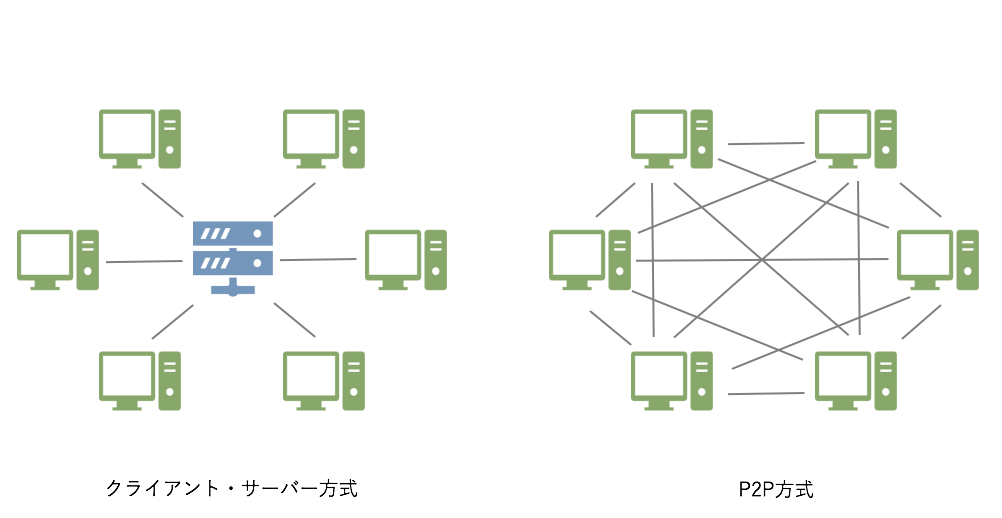
\includegraphics[width=100mm]{image/P2P.png}
 \caption{クライアント・サーバ方式とP2P方式のネットワークイメージ}
 \label{P2P}
\end{figure}

\subsection{デジタル署名とアドレス}
デジタル署名とは、あるメッセージが署名した人によって作られたかを検証する仕組みである。
ここでは「Aが自分の3BTC(Bitcoin)を使いたい」と主張する時に、それが本当にAの発言であるかを担保するのがこのデジタル署名の役割である。
代表的なブロックチェーンであるBitcoinやEthereumではECDSA(楕円曲線DSA, Elliptic Curve Digital Signature Algorithm)を利用しており、これについて説明を述べる。
\begin{equation}
y^2 = x^3 + ax + b
\end{equation}
以上が楕円曲線について一般的に表される式である。
この中でもBitcoinやEthereumが用いる規格であるsecp256k1曲線はa=0, b=7であるため、以上の方程式は
\begin{equation}
y^2 = x^3 + 7
\end{equation}
上記のように表される。
これをxy座標で表すと、以下\ref{ecdsa2}\footnote{\url{https://zoom-blc.com/what-is-ecdsa} (2018年1月23日確認) より引用}のようになる。
\begin{figure}[htbp]
 \centering
  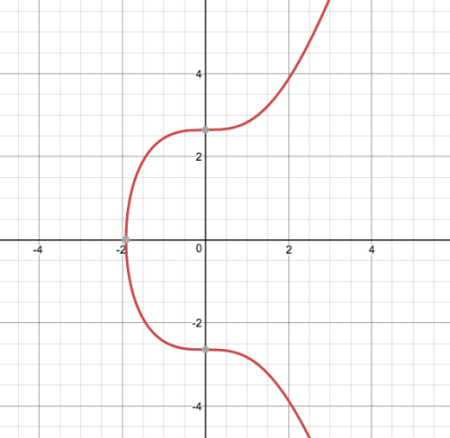
\includegraphics[width=60mm]{image/ecdsa2.png}
 \caption{$y^2 = x^3 + 7$の楕円曲線}
 \label{ecdsa2}
\end{figure}
また楕円曲線の加算の定義として、点Aと点Bを加算することを考える。
この時、加算後の座標は点Aと点Bとを通る直線のもう一つの交点のx軸に関して対称移動させた点である。
したがって点Aと点Bが同一座標の点Gであるとき、その接線と楕円曲線との交点をx軸に関して対称移動させた点は
G + G = 2G
となる。
secp256k1はGのベースポイントを定めており、そこから秘密鍵rを掛け合わせたrGが公開鍵となる。
この時、楕円曲線上の離散対数問題によって秘密鍵から公開鍵を導出することは容易であるが、逆の公開鍵から秘密鍵を導出することは難しいことが知られている。
この秘密鍵を使い、「自分のBitcoinを使いたい」と主張することによって、利用者は自分のBitcoinを使用する事が可能となる。
この主張を行う際の署名値は以下の式によって導かれる。
\begin{equation}
S=\frac{h+kR}{q}{(mod p)}
\end{equation}
\begin{list}{}{}
\item q:一回のみ使われる乱数(\(1 \leq q \leq 2^256-2^32-977\))
\item h:取引情報のハッシュ値
\item k:送信者の秘密鍵
\item R:一時的な公開鍵のx座標
\item p:楕円曲線のx座標がこれより大きくならないための値で素数
\end{list}

そしてこれらの値のうち、SとRが署名となり、ブロックチェーン上で周知される。
この主張が本人のみ知り得る秘密鍵を使って行われたものかを確認する際は、以下の式を使って検証する。
\begin{equation}
Q=\frac{hG}{S}+\frac{RK}{S}{(mod p)}
\end{equation}

\begin{list}{}{}
\item S, Q, R:送信者から受け取った署名
\item h:取引情報のハッシュ値
\item G:secp256k1のベースポイント
\item K:送信者の公開鍵
\item p:楕円曲線のx座標がこれより大きくならないための値で素数
\end{list}

以上の式において、Qのx座標が送信者が送信したRの座標と一致する時、この署名は正しいものであると検証される。
また、この公開鍵をBitcoinではHASH160\UTF{00B7}EthereumではKeccak256ベースのハッシュ関数によってそれぞれハッシュ化し、Ethereumではそのハッシュ値の末尾20バイトを抜き出したものがアドレスとして使われる。
そして「そのアドレスに対して、3BTCを送金する」と主張できるようになり、このアドレスの管理者(つまり元の公開鍵や秘密鍵を持っている者)がその後、「ここで受け取った3BTCを使う」と主張できるようになるのだ。
(!!!後に参照する図を挿入のこと!)

\subsection{トランザクション}
ここでは、Bitcoinを例にとトランザクションについて説明を行う。
ブロックチェーン上の記録は、全てトランザクションという単位毎に格納される。
つまり、「AがBに3BTCを渡した」という記録が一つのトランザクションに格納されるということだ。
このトランザクションはインプット部分とアウトプット部分、そしてその他の部分が存在する。
インプットには、当該トランザクションのトークンの出所が存在している。
例えば、「Aが3BTCを使う」と申し出たとしよう。
この時、ネットワーク全体が「Aは3BTC以上持っている」ということが分からないと、Aが3BTC使うという行為は認められない。
ここで「3BTC以上持っている」ということは、換言すると「3BTC以上を誰かから送金された過去があり、そのBTCは未だに使用されていない」ということである。
この「未だに使用されていなく、その所有者が未だ使える状態」のトランザクションのことをBitcoinではUTXO(Unspent Transaction Output)と呼ぶ。
このUTXOを使おうとする時は、トランザクションのインプットにUTXOの存在する場所を明示することで、UTXOを使う事ができる。
つまり、インプットはトランザクションの送金における払い手に当たる情報が入る部分と言える。
次に、アウトプットについて説明する。
アウトプットはトランザクションの送金における受け取り手に当たる情報が入る部分である。
前項で述べたように、受け取り手の情報はアドレスによって表される。
したがって、「AがBに3BTCを渡した」あとで未だにBがこれを使っていない状態の時、このトランザクションのアウトプットの署名欄にはBitcoinアドレスが存在している。
その後、「BがCに3BTCを渡した」とすると、先ほどBitcoinアドレスが書かれていた署名欄にはBitcoinアドレスの素となった公開鍵とこの公開鍵に対応する署名値が代入される。
つまり、あるアウトプットがUTXOであるか否かの判断はこの署名欄にBitcoinアドレスがあるか公開鍵と署名値が存在するかの違いによって行われる。
このようにしてトランザクションは管理される。
このトランザクション(tx)とUTXOの関係を示した図を下図\ref{UTXO}\footnote{\url{https://zoom-blc.com/utxo-bitcoina} (2018年1月23日確認) より引用、一部改変}で示す。
\begin{figure}[htbp]
 \centering
  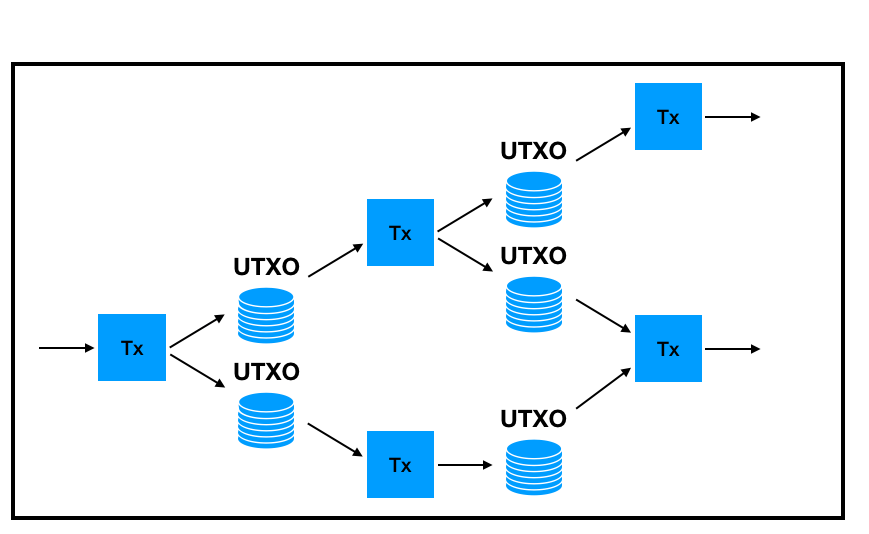
\includegraphics[width=60mm]{image/UTXO.png}
 \caption{トランザクション(tx)とUTXOとの関係}
 \label{UTXO}
\end{figure}

\subsection{ブロックとマイニング}
ここではブロックとマイニングについて説明を行う。 \\
ブロックチェーン技術は情報の記録を単一の歴史を共有することによって、参加者の合意できる台帳管理を行おうとする技術である。
この単一の歴史を刻む歴史書の1ページが1ブロックに当たる。
現在のBitcoinでは10分に1回、Ethereumでは15秒に1回、それぞれのペースで新しいブロックが生成される。
このブロックにはトランザクションが0個以上含まれており、その処理内容が単一の歴史として刻まれる。
そしてブロックチェーン技術はこの方式によって、二重支払い問題を解決している。
Aが3BTCを持っている時、同時に「AがBに3BTCを払う」と「AがCに3BTC払う」というトランザクションを発行しようとしたとする。
しかし、ブロックが生成される際にのみ送金の処理は行われるため、ネットワークの遅延等の影響によって二つのトランザクションが承認されることはあり得ない。
また、各々のブロックはヘッダに前のブロック情報をまとめたハッシュ値を持っており、どのブロックの次に繋げられたブロックであるかを明示している。
このブロックがチェーンのように何個も連なることによって、ブロックチェーンという分散管理台帳が形成されていく。 
その様子について、下図\ref{block}\footnote{\url{https://github.com/ethereum/wiki/wiki/White-Paper} (2018年1月24日確認) より引用}に示す。
\begin{figure}[htbp]
 \centering
  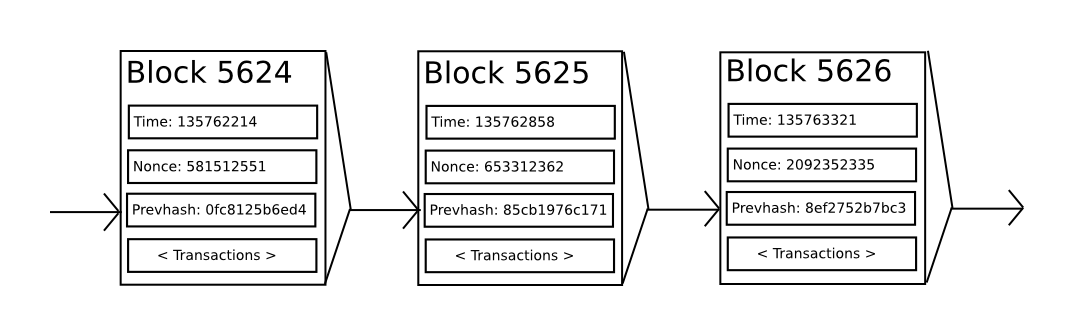
\includegraphics[width=120mm]{image/block.png}
 \caption{ハッシュ値により繋がるブロックチェーン }
 \label{block}
\end{figure}
そしてこのブロックが生成される際に行われることが、マイニングと呼ばれる行為である。そしてブロックの生成を行おうとする者をマイナーと呼ぶ。
ブロック情報をまとめたハッシュ値の中には、ナンスと呼ばれるブロックのマイナーが付加する32bitの数値が存在する。
このナンスを含めたハッシュ値が、一定の数だけ頭に0を持つようにすることによって、そのブロックは正当なブロックであると承認されるようになっている。
例えば、Bitcoinのメインネットワークにおいて553582番目に生成されたブロックの情報について見てみる。
以下はBitcoinの現在の統計情報などを提供しているサイト、https://www.blockchain.com/ja/ から取得した情報である。
すると、ハッシュ値は「0000000000000000001b0218ca2b54e9809b5d948864c5bd1e657e5aa09f438f」となっている。
そしてこの時のナンスの値は「4142738813」となっている。
ブロックの持つトランザクションのハッシュ値などの情報に、このナンス値を足したところ、このように頭にいくつもの0がつくハッシュ値を見つけ出せたのである。
この時この様々なナンスの値を取り付け、0が頭に一定数以上つくハッシュ値を見つけ出す行為について、マイニングと呼ぶ。
そしてこのマイニングという行為によって、ブロックチェーンにおける改竄可能性を防いでいるのだ。
現在(2018-12-13 00:46:30)、マイニングは16進数において頭の18文字に0が続く場合、ブロックが生成されるようになっている。
つまり、最新より一つ前のブロックのハッシュ値をブロックに含めて\(16^18\)回の演算を行うことで最新のブロックを無効にでき、自分の思い通りのブロックを提出する事ができる。
しかし、2つ前のブロックを変更しようとするときはどうだろう。 \\
Bitcoinの各参加者は、ブロックがもっとも長く連なったブロックチェーンを信用するように設計されている。
つまり2つ前を変更するには、新しく2つ分のブロックを生成しなくてはならないのだ。
この時に必要な計算量は\(16^(18\times2) \)となり、難易度は格段に上昇する。
これがさらに3つ前、4つ前..となっていくと、事実上変更は不可能となる。
よって3BTCを払い、その対価としてのサービスを受けたのちにその支払ったBTCを取り返すために新しいブロックを作り直す行為は、ブロックが一定数以上深くなった場合においては不可能である。
つまり理論的にブロックの改竄は可能であるが、それは実際にはそれを行うことは極めて難しいということである。
これがブロックチェーンの参加者が公開台帳を信用する理由であり、改竄耐性を持つという理由である。
そしてマイナーがこのマイニングを行う動機はマイニングを成功した時に成功報酬がもらえることである。
この成功報酬はブロック高によって決められており、最初は50BTCで始まり、2018年12月現在では12.5BTCである。 \\
また、ブロックは過半数の計算能力がある攻撃者によって占められた場合、誤った処理のなされたブロックの先に攻撃者のマイニングによるブロックがつながるようになってしまう可能性がある。
これは51\%攻撃と呼ばれ、大きな計算能力を持たないネットワークの暗号通貨はこの攻撃を受けやすい。
このようにしてブロックは生成され、ブロックチェーンは管理される。

\section{問題点}
ここでは、前半の2項でブロックチェーン技術に関する固有の問題点を述べる。
その後、後半の2項で現在のブロックチェーン事情に関する問題点を述べる。

\subsection{スケーラビリティ}
ここではブロックチェーンで管理することによる、トランザクション処理数に関するスケーラビリティの少なさについて述べる。
Bitcoinでは1ブロックに含める事が可能なデータ量は1MBとなっている。
このデータ量の中にトランザクションに関するデータを含めなくてはならないため、1ブロックで処理できるトランザクションの数は限られている。
そしてブロックの生成ペースは平均で10分に1回になるように調整されるため、処理できるトランザクションの数は時間当たりで一定であると言える。
つまりBitcoinを100人が使おうが、100万人が使おうが、同じだけの処理能力しか存在しないのである。
例えばWebサービスであれば、受け付けるリクエストに対する処理能力を上げる方法はたくさんある。
Webサーバの台数を増やし、ロードバランサで負荷を振り分ける。
DBを分散処理させ、データモデリングを見直してよりレスポンスの速いDBにする。
JavaScriptを後から読むようにし、思い画像は最初のトップページ範囲を表示してから順にAjaxで取得する。
など、様々な方策を打てる。
しかし、ブロックチェーンは時間をかけてマイニングを行い、複数のチェーンが同時並行で存在していくことを防いでいる。
もし3秒に1回のペースでブロックが生成される場合、同じ長さのチェーンが大量にできてしまい、どれが本当の台帳とみなして良いかわからなくなる。
また、ブロックには一定のサイズしか入らないことで最新のブロックが変更された時の巻き戻されるトランザクションの数を減らしている。
もし大量のトランザクションを1つのブロックに入れた場合、それはブロックを広報する際の遅延が生じる。
この時、最新のブロックからマイニングを行いたいマイナーは、ブロックの遅延によって不利を受ける。
これが続いた場合、マイナーが少なくなり、マイナーの一極集中を招く恐れがある。
このことによる弊害については3.2.4にて後述する。
つまり、仕組みそのものに固有のスケーラブルになり得ない要素が含まれているのだ。
勿論、マイニングには参加者が多い方がマシンパワーが大きいので、変更されにくいブロックを生成する事が可能である。
しかしながら、それは改竄耐性が上がるのみであり、トランザクションの処理能力は上がらない。
どれだけ沢山の参加者が増えたとしても、それはセキュリティ性を高めるために使われてスループットを犠牲にしている、ここにブロックチェーンの大きな問題点の一つが存在する。

\subsection{手数料とマイクロペイメント}
全世界では大量のトランザクションが生成されている。
従って、生成された全てのトランザクションが直ぐに最新のブロックに入るとは限らない。
この時、早くマイナーにブロックへ入れて貰うため、トランザクションの送信元は手数料を設定することができる。
この手数料はマイナーが得る成功報酬にプラスして、マイナーへと渡る。
よって、より多くの手数料を指定した方が早くトランザクションが処理される可能性が高まるのだ。
またブロックサイズの上限が決まっているため、トランザクションの大きさが大きい程、多くの手数料がマイナーへのインセンティブに必要となる。
1MBの内500KBを使うトランザクションを処理して0.01BTCの手数料のトランザクションと、1MBの内50KBを使うトランザクションを処理して0.01BTCの手数料のトランザクションとでは残りのブロックに入れられるトランザクションの大きさが変わってくるためである。
残りでより大きなトランザクションを捌ける方が、より多くの手数料を獲得できるためである。
しかしこの仕組みは、小さな買い物に使うためには適していない。
手数料はトランザクションベースで決まるため、少額の支払いであれば手数料が少なくて済むという性質のものではないためである。
つまり、Bitcoinで10円にあたる飴を買う際も1000万円にあたる高級車を買う際も、同じ速度で処理してもらうには同じ手数料が必要なのだ。
よってここまで記したのブロックチェーン技術では、マイクロペイメント(少額取引)には適さないという問題点がある。

\subsection{マイナーの一極集中}
ブロックはブロックチェーンにおける歴史書の1ページであり、マイナーはそのブロックを承認する役割を持っている。
即ち、マイナーは取引の歴史の承認者、ブロックチェーンの管理者と換言できる。
そしてそもそも、ブロックチェーンは完全に分散された記録システムであった。
中央集権な機関が存在しないので、その完全に透明性が保たれたプラットフォームを信用する人が参加するものとして作られた。
しかしながらこの前提を覆すようなことがBitcoinでは起こったと、Bitcoinのコア開発者でBlockstreamの共同設立者であるPieter Wuille氏は言う。
マイナーの中にはマイニングプールと呼ばれるものを作り、ブロックを生成している集団がある。
彼らは自宅のPCなどでマイニングをしたいものの、成功する確率が少ないので大勢でマイニングを行っている。
そして例えば各人の計算能力が同じ100人で12.5BTCを採掘した場合は、1人あたり0.125BTCずつ分配する。
このいくつかのマイニングプール間で、生成したブロックを送信する前にブロックヘッダのみを共有しているようなのだ。
これにより、情報を共有するマイニングプールは他のマイナーよりも早くマイニングに取りかかることができる。
これは計算能力を信用しているのではなく、共有の相手のマイニングプールを社会的に信用していることであり、これはBitcoinの基本理念に反する。
それと同時に、これらのマイニングプール間でのマイニングが有利となり、他のマイナーがマイニングに参加する際に不利となってしまう。
ここで、これからマイニング参加するにはこのマイニングプールに所属する方法が一番良い方法となる可能性がある。
その際マイナーは歴史の承認者であるため、一極集中するとその間でメインのBitcoinとは別の取り決めを作ってしまい、それがBitcoinのルールとなってしまう可能性がある。
この時、本来の目的と離れてBitcoinに中央集権的な機関が存在してしまう可能性がある。 \\
また、51\%攻撃がいくつかのマイナーの協力によって行われてしまう可能性がある。
下図\ref{MiningPool}\footnote{\url{https://www.blockchain.com/pools?timespan=4days} (2018年1月24日確認) より引用}が現在(2019年1月24日2時13分)から4日間に採掘されたブロックにおける、マイニングプールの割合である。
\begin{figure}[htbp]
 \centering
  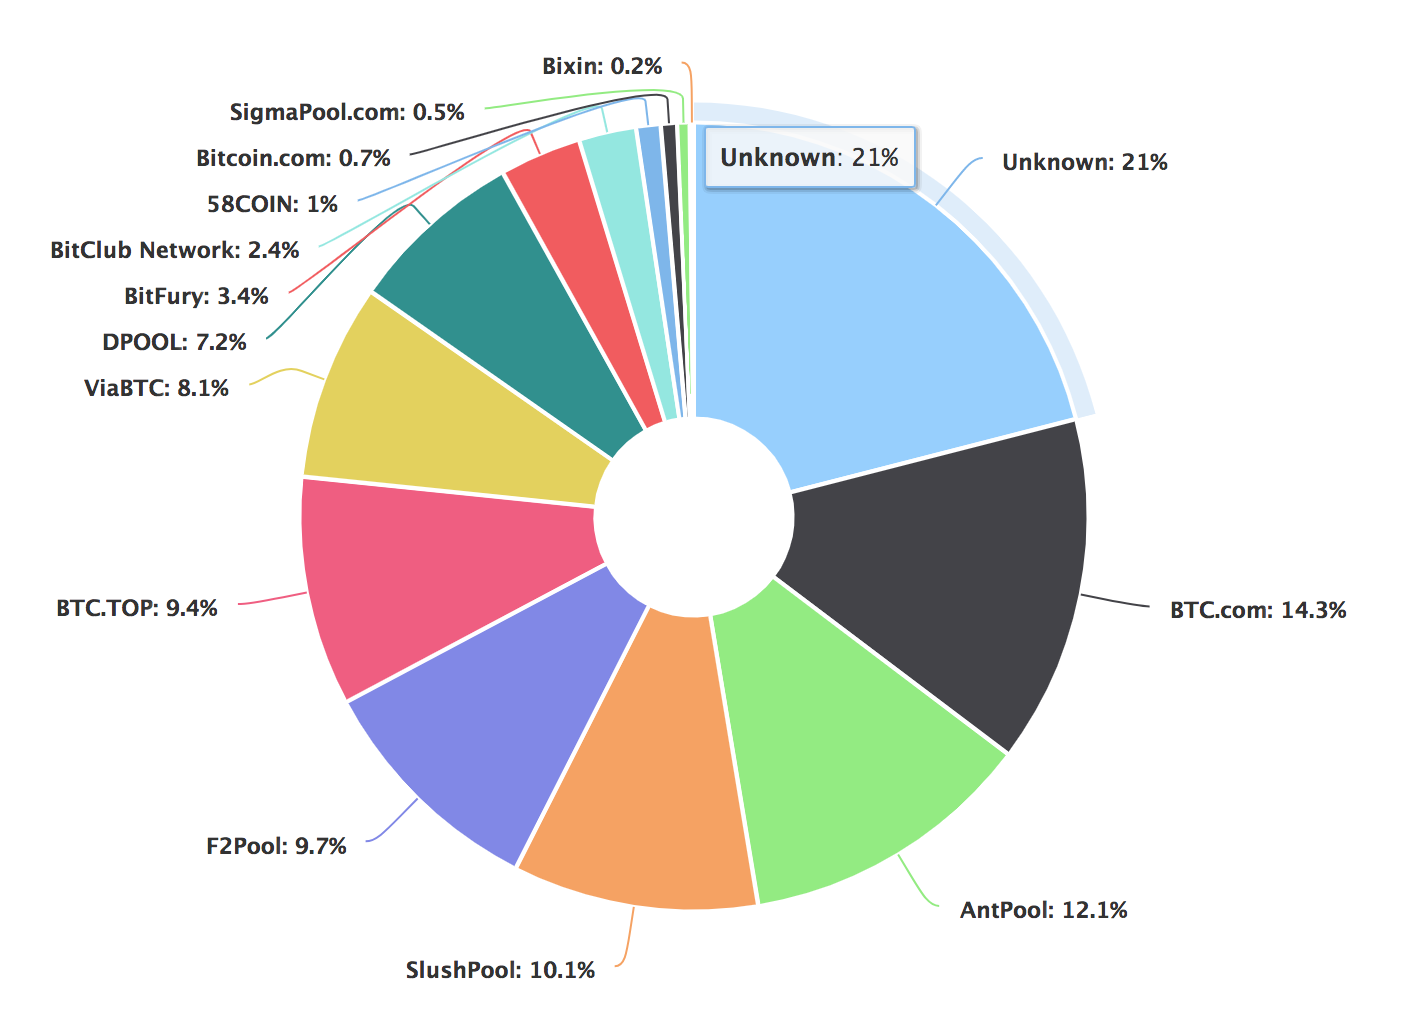
\includegraphics[width=60mm]{image/MiningPool.png}
 \caption{トランザクション(tx)とUTXOとの関係}
 \label{MiningPool}
\end{figure}
この図より読み取ると、最低で5つのマイニングプールが協力した場合、51\%攻撃は可能である。
これはビットコインネットワークの信頼性を低下させるものである。 \\
以上の理由から、マイナーの一極集中は望ましいことではなく、現在のBitcoinを取り巻く状況の問題点の一つである。

\subsection{現在のOSSブロックチェーンの運営}
"Decentralization in crypto is a myth. It is a system more centralized than North Korea: miners are centralized, exchanges are centralized, developers are centralized dictators"
「暗号通貨が中央集権的でないと言うのは神話である。そのシステムは北朝鮮よりも中央集権的である。マイナーは中央集権的で、交換所は中央集権的で、開発者は中央集権化された独裁者である。」
以上の言葉はニューヨーク大学のNouriel Roubini教授がtwitterで発言した言葉である。
確かに、現在のブロックチェーンはパブリック型であってもその仕様の決められ方は決して民主的なものではない。
Ethereumは2019年の1月にハードフォークが行われることが決まったが、これは開発者会議によって決まったものだ。
それ以前でも、EthereumはThe DAO事件の時のハードフォークから中央集権的であると批判を集めてきた。
The DAOというEthereum上で動くトークンの資金集めに150億円分のEthereumが集められた。
しかし、Ethereum上で動かすsolidityと言う言語のフォールバック関数の仕様に関しての見落としがあり、3分の1が攻撃者によって抜き取られてしまった。
その際、Ethereumコミュニティは歴史書であるブロックチェーンの巻き戻しを行い、攻撃者が利益を得ることを阻止した。
このような対策が一プロジェクトのバグに対して行われること自体が、中央集権的であることの証左である。
ここにマイナーやETH(Ethereumの通貨単位)を持っている人間の意思は反映されていない。
マイナーの件に関しては前項で述べたものがそのままこのツイートの論拠となる。
このように、現在のOSSブロックチェーンはパブリック型と謳いつつ、とても中央集権的であるという側面を持っている。

\section{オフチェーン技術}
ここではオフチェーン技術について述べる。
今までのブロックチェーンに関する説明はこれに対応してオンチェーンと呼ばれることがある。
オンチェーンはトランザクションの制限が厳しく、全世界で使われる通過の処理が10分に1回しか行われない。
Bitcoinが始まって以来、一日のトランザクションが45万を超えたことはない。
これは、秒間5.2トランザクション以上が処理されたことがない計算になる。
VISAを始めとした決済システムは遥かに多いTPS(Transaction Per Second)を実現しており、世界中の決済を目的とするには5TPSは明らかに少ない数字である。
この制約を緩やかにするため、オフチェーン技術と総称される技術が存在している。
例えば1曲100BTCで楽曲を配信するサービスを考えてみる。
最初に、ユーザは使いたいBTCをオンチェーン上にデポジットする。
10曲分配信サービスを受けたいと予定したすると、1000BTCをデポジットする契約をトランザクションとして広報する。
その後1曲の配信サービスを受けるとき、支払い側は100BTC分を払うという署名を行ったトランザクションを受け取り側へ送る。
受け取り手はこのトランザクションを確認次第、1曲の楽曲を配信する。
そして支払い側がもう1曲楽曲が欲しい時は今度は200BTCを払う署名を行ったトランザクションを受け取り側へ送る。
というこの繰り返しを行い、もう支払い側が要らないと思った時、このオフチェーンでのやり取りを終える。
この時の実際の操作としては、受け取り側が精算する旨をトランザクションとして広報することを行う。
そしてもし6曲の配信サービスを受けた時、600BTCが受け取り側に、400BTCが支払い側に支払われる。
この時、最初と最後の2つのトランザクションのみオンチェーンには広報したが、実際にはオフチェーンによって6曲分の支払いがなされている。
オンチェーンのみでは6つのトランザクションが必要なところを2つのトランザクションのみで同じ機能を提供できたということである。
これがオフチェーン技術の概略であり、これに対する細かな実装はブロックチェーンの種類によって違う。
各々がBitcoinとEthereumのオフチェーン技術の一つである、ペイメントチャネル技術とμRaiden技術については後の3.4.3項と3.5.4項にて行う。

\section{Bitcoin}
ここではブロックチェーン技術を使って作られた最初の実装物であるBitcoinについて述べる。
3.1節で説明したことと重複することが多いが、のちのEthereumと対比するために述べる。
通貨単位はBTCである。

\subsection{トランザクションベースの一元管理}
Bitcoinは全てトランザクションベースで管理される。
3.1.2項で述べたように、自分のBTCを使いたい時はそのBTCをもらった過去のトランザクションを指定する。
そしてそのトランザクションを指定してBTCを使った過去がないことを承認ノードが確認(UTXOであることを確認)した上で、そのBTCは使用される。
ここで、仮に10BTCを貰ったトランザクションを使って3BTCを使いたいとする。
すると支払い側は生成されるトランザクションは3BTCを支払い相手へ渡し、残りの7BTCは自分のアドレスへ送るように指定することで3BTCのみを使うことが可能となる。
この工夫が一般的である理由は、トランザクションベースの一元管理であることに存在する。
もし7BTCを明示しない場合、お釣りの7BTCがそのまま送信者のアドレスに紐づけられたままできるのであればトランザクションのサイズを減らし、トランザクション送信の際の手数料を少なくできる。
お釣りのアドレスを指定することは送信相手を複数指定するためにトランザクションのサイズが大きくなることを招き、このことがトランザクション送信の際の手数料増大を招くためだ。
もしアカウントベースでBitcoinが管理されていれば、この方式を行うことに一定の負のインセンティブが存在する。
また、トランザクションベース管理ではこのお釣りであるという情報を秘匿する工夫も考えられている。
もし同じBitcoinアドレスへ7BTCを送った場合はこの7BTCがお釣りであることが明確であり、本来は公開されるべきでない支払い情報の一部が全世界にバラされてしまう心配がある。
よって、これに対する一般的対策としてBIP(Bitcoin Improvement Proposal)-32で提案された、拡張鍵生成が知られている。
これはチェーンコードやインデックスの数字を用い、新しく秘密鍵\UTF{00B7}公開鍵\UTF{00B7}Bitcoinアドレスを生成する方法の一般的方法である。
これを使うことで、同じく自分が管理しているアドレスでありながらマイナーや他の参加者からはどちらがお釣りでどちらが本来の支払いに使われたのか、あるいはどちらも別々の支払いに使われたのかが分からなくなる。
このようにして、支払い情報についてなるべく公開されないような工夫が一般的に行われている。
また、Bitcoinが徹頭徹尾トランザクションベースで管理されていることがこれらの振る舞いや工夫から分かる。

\subsection{script言語とチューリング不完全}
Bitcoinの署名に関して、具体的な方法について今まで言及してこなかったが、これがscript言語と呼ばれるもので行われているという具体的プロセスをここで記す。
UTXOの使用時、script言語と呼ばれる言語によって記述されたプログラムが正を返す時、そのUTXOは使用可能となる。
Bitcoinの使用例としてもっとも代表的である、Bitcoinをあるアドレスからあるアドレスへ移動させる場合を考える。
その際のプログラムは以下のようになる。
\begin{lstlisting}[caption=script言語,label=scripting]
<sig> <pubK> DUP HASH160 <pubKHash> EQUALVERIFY CHECKSIG
\end{lstlisting}
\begin{list}{}{}
\item \verb|<|sig\verb|>|:秘密鍵でトランザクションに署名したもの
\item \verb|<|pubK\verb|>|:公開鍵情報
\item DUP:一つ前の内容をコピーする命令
\item HASH160:公開鍵からアドレスをBASE58でデコードしたものを導く関数
\item \verb|<|pubKHash\verb|>|:アドレスをBASE58でデコードしたもの
\item EQUALVERIFY:スタックに積まれている一つ前ともう一つ前が同じであることを確認する命令。異なればその時点でプログラム全体の返り値がFalseとなる。
\item CHECKSIG:二つ前の署名値が一つ前の公開鍵情報に対して正しいか否かを判断する。
\end{list}

このscript言語は逆ローランド記法であり、順に命令がスタックに積まれて実行されていく。
なお、この時トランザクションのアウトプットに記述される、トランザクションをロックするためのプログラムが以下である。
\begin{lstlisting}[caption=ロックを行うscript言語,label=scripting-lock]
DUP <HASH160> <pubKHash> EQUALVERIFY CHECKSIG
\end{lstlisting}
そしてインプットに記述されるトランザクションをアンロックするためのプログラムが以下である。
\begin{lstlisting}[caption=アンロックを行うscript言語,label=scripting-unlock]
<sig> <pubK>
\end{lstlisting}
つまり、「アンロックのためのプログラム」と「ロックのためのスクリプト」をこの順番で続けて実行することでトランザクションへの署名が正しいかの判断は行われる。
以下にその時の様子を示す。
\begin{enumerate}
\item \verb|<|sig\verb|>|がスタックに積まれる
\item \verb|<|pubK\verb|>|がスタックに積まれる
\item DUPによって\verb|<|pubK\verb|>|が複製される
\item HASH160によって3番目で複製された公開鍵情報がアドレスのデコードされた状態の値になり、スタックに積まれる
\item \verb|<|pubKHash\verb|>|がスタックに積まれる
\item EQUALVERIFYによって4番目でハッシュ化されてスタックに積まれたものと5番目でスタックに積まれたものとを比較する。同じであった場合は実行中のプログラムが続行され、異なっていた場合は実行中のプログラムは中止する。
\item CHECKSIGによって、1番目でスタックに積まれた署名値と2番目でスタックに積まれた公開鍵情報を検証し、正しいものであれば真を返し、間違っていれば偽を返す。
\end{enumerate}
以上がscript言語の実行内容である。
また、このscript言語の特徴として、チューリング不完全であることが挙げられる。
このことにより、チューリング完全である時と比べてセキュリティホールが少なく済むことが知られている。
その一方で、このスクリプト言語によりユーザが望む様々な処理が実現できるとは限らない。

\subsection{ペイメントチャネル}
Bitcoinにおけるオフチェーン技術であるペイメントチャネルは、トランザクションの持つロックタイム機能とマルチシグ機能を併用して実現される。
ロックタイムとは、定めた時間になった時までそのトランザクションが実行されない機能のことである。
マルチシグとは、あるUTXOを使う際に複数の署名値が要求できる機能のことで、「N of M のトランザクション」などと表される。
これはM個のアドレスの内、N個のアドレスの署名値が必要となるUTXOであるということを示す。
例えばAが消費者\UTF{00B7}Bが販売者とし、AからBへ1000BTCのデポジットを最初のトランザクションとして持っておき、そこから100BTCずつで楽曲を買うことのできる状況を想定してみる。
\begin{enumerate}
\item AはAとBの署名値が必要な 2 of 2 のマルチシグのトランザクションを生成し、ブロードキャストする。同時に、2of2のマルチシグなのでBobが音信不通になった時の保障のため、Bが何も行わない場合Aに全てのBTCが戻るトランザクションをマルチシグのインプットから提出する。この際、この戻るトランザクションに関しては一定期間が過ぎた後に実行されるようにロックタイムを掛けておく。
\item Aが1曲の楽曲を買うため、マルチシグのトランザクションにAのみが署名し、アウトプットとしてAに900BTC\UTF{00B7}Bに100BTCを支払うトランザクションをBへ送る。
\item Aが更に1曲の楽曲を買うため、マルチシグのトランザクションにAのみが署名し、アウトプットとしてAに800BTC\UTF{00B7}Bに200BTCを支払うトランザクションをBへ送る。
\end{enumerate}
この時、Bは自分に100BTCでも200BTCでも送ることが可能な権利を持つが、通常は200BTCを貰う方を選択する。
このようにしてチェーンの外での取引が実現される。
そして、Aが払うという範囲においては、Bの方からAへBTCを送ることも可能である。
ここでは先ほどの例のシチュエーションにプラスして、1ヶ月ごとに抽選があり、それに当たると50BTCが帰ってくるという場合を想定してみる。
\begin{enumerate}
\item AはAとBの署名値が必要な 2 of 2 のマルチシグのトランザクションを生成し、ブロードキャストする。同時に、2of2のマルチシグなのでBobが音信不通になった時の保障のため、Bが何も行わない場合Aに全てのBTCが戻るトランザクションをマルチシグのインプットから提出する。この際、この戻るトランザクションに関しては一定期間が過ぎた後に実行されるようにロックタイムを掛けておく。
\item Aが2曲の楽曲を買うため、マルチシグのトランザクションにAのみが署名し、アウトプットとしてAに800BTC\UTF{00B7}AとBのマルチシグに200BTCを支払うトランザクションをBへ送る。そして同時に、AとBのマルチシグにAが署名を行い、そのマルチシグからBへ送るようにする。この際、Bへのトランザクションには1番目に生成したロックタイムより前に設定されたロックタイムを設定しておき、Bのアドレスは今回のみ使われる一時的なアドレスを使用する。
\item ここでAが抽選にあたり、BはAへ50BTCを支払おうとする。しかしAが850BTCを持ち、Bが150BTCを持つトランザクションを作ったとしても、Bが先ほどの200BTCを貰えるトランザクションを提出しない保証はない。そこで、Bは一時的に利用したアドレスの秘密鍵をAへ送る。これによって、BはAに前の契約より少ないBTCの契約に同意したことを示す。
\end{enumerate}
もしBが200BTCのトランザクションをブロードキャストした場合は、Aはその後に続くトランザクションがロックタイムに到達する以前にAとB(一時的なアドレス)のマルチシグからAへ150BTCを送るトランザクションを発行できるので、Bはそのためのトランザクションをブロードキャストしない。
Bがブロードキャストしなければ、Aに全額が渡るトランザクションはインプットが存在しなくなるためだ。
このようにしてBitcoinのオフチェーンは実現される。

\section{Ethereum}
ここでは本研究で用いるブロックチェーン技術であるEthereumについて述べる。
3.4.1と3.5.1が、3.4.2と3.5.3が、3.5.3と3.5.4がそれぞれの特徴に対応している。
通貨単位はETHである。

\subsection{トランザクションベースとアカウントベースの二元管理}
Ethereumはトランザクションに基き、アカウント毎にEthereumを管理している。
もちろん、Bitcoinと同様に「3ETHを持っている」=「3ETHを過去に送ってもらったことがある」という考えのもと、Aが3ETH持つにはAに3ETHを送ったトランザクションが存在しなくてはならない。
しかし、このトランザクションの結果、Aの持つアドレスに3ETHが紐づくのだ。
つまり、3ETHを使う際は前のトランザクションに署名をして使うのではなく、「3ETH使います」ということをAのアカウントの署名で提出すれば3ETHが使えることになるのだ。
これは面倒なお釣りの処理を行う必要も無くす。
Aが3ETH持っていて、Bに2ETHを送信した時、別途自分用のお釣りのアドレスを用意せずとも残りの1ETHは自分のアドレスに紐づいているのだ。
問題点としては、ハードフォークが起こった時にバージョンやChainIDを変更ことができないことが起こってしまうと、リプレイアタックの攻撃の可能性があることである。
The DAO事件を発端に、Ethereumは急遽EthereumとEthereum Classicにハードフォークすることとなった。
ブロックの巻き戻しを行うか否かで意見が割れ、巻き戻したほうがEthereum、巻き戻さなかった方がEhtereum Classicとなった。
そしてこの事件より前から所持していたEthereumを送金しようとすると、それと同じトランザクションをEthereum Classicネットワークでも送信できるようになる。
よってこの際、Ethereum Classicは持っている人の意思とは無関係にEthereum送金と同時にEthereum Classicも送金されてしまう可能性を持ってしまうのだ。
これはトランザクションベースの一元管理では起こり得なかったことである。
アカウントベースでの管理を加えたことは、複雑な処理を可能にしたと同時に、セキュリティ面では厄介な問題を引き起こす原因を作った。

\subsection{スマートコントラクト}
EthereumのアドレスはEOA(Externally Owned Account)アドレスとコントラクトアドレスが存在する。
Bitcoinのアドレスと同様に、所有者に紐付くアドレスがEOAアドレスである。
EOAアドレスからは採掘や送金などを行うことができる。
Bitcoinアドレスと異なる存在が、コントラクトアドレスである。
Ethereumではスマートコントラクトと呼ばれるものが作成できる。
これは人が持つものではなく、コードとして定義された関数である。
Ethereumはそれそのものがブロックチェーンでありながら、Ethereumネットワーク上でコードによって支配された世界を築く土台であろうとしている。
そしてコードによって支配された世界に当たるものがこのスマートコントラクトである。
また、このスマートコントラクトにつけられたEthereumネットワーク上でのアドレスがコントラクトアドレスとなる。
スマートコントラクトはよりフレキシブルな非中央集権の世界を作ることができる。
Bitcoinは金にあたるトークンのやりとりのみが行われているのみだった。
その一方で、スマートコントラクトは例えば管理会社のいないギャンブル市場を作ることが出来るのだ。
ここではAugurというEthereum上で動いているスマートコントラクトを例に述べる。
Augurの参加者はまず、賭けに関するトピックを生成し、それをブロードキャストする。
それに興味を持った参加者が賭けを行うため、作成されたトピックに存在する選択肢から一つを選び、賭けたい量のAugurトークンを賭ける。
もしこれが競馬のレースであったとするならば、レース終了後にこの事実を認定するフェーズに入る。
事実はレース終了後に選択肢の中から正しい選択肢に対して賭けることで行われ、レース終了後でもっとも多く賭けられた選択肢が事実として認定される。
その後、争議ラウンドが設けられ、これに対する異議申し立てを行える期間がある。
そして最終的な決着を見た結果に基づいて払戻金が支払われるという仕組みになっている。
この際、トピックを生成することに関してインセンティブとなるように生成者には一定のAugurトークンが支払われる仕組みを持っている。
さらに、レース後の投票においても最終的な結論に至らない場合、チェーンがフォークすることも前提にした仕組みを持っている。
そしてこの賭けのサービスを応用すると、保険機構も作れるのだ。
「Aさんが怪我を負うか」というトピックににAさんがずっと「怪我を負う」賭け続け、Aさん以外が「怪我を負わない」に賭け続けるとする。
するとAさんが怪我を負った時、賭けに勝ったお金として保険金に当たる今まで「怪我を負う」に賭け続けた失ったトークンが戻ってくるのだ。
この場合、怪我の認定について誰が行うかなどの曖昧な点が残されているが、原理としては行うことが出来る。
このように、スマートコントラクトは単なる送金よりもフレキシブルなコードによって支配された非中央集権の世界を作ることの可能な技術なのだ。

\subsection{solidityとチューリング完全}
solidityは前述のスマートコントラクトを記述する言語である。
そして、フレキシブルな世界実現のため、solidityはチューリング完全な言語となっている。
例えば、貨幣のような価値を持つトークンの存在を前提としたスマートコントラクトにはERC20という基準が存在するが、これについての関数とイベント宣言の記法について見てみる。
これは、このERC20に沿っていれば、Ethereumネットワーク上でトークンとしての役割を果たせると言えるものである。
\begin{lstlisting}[caption=ERC20を満たすために必要な関数とイベントの宣言文,label=ERC20-criteria]
function totalSupply() constant returns (uint256 totalSupply);
function balanceOf(address _owner) constant returns (uint256 balance);
function transfer(address _to, uint256 _value) returns (bool success);
function transferFrom(address _from, address _to, uint256 _value) returns (bool success);
function approve(address _spender, uint256 _value) returns (bool success);
function allowance(address _owner, address _spender) constant returns (uint256 remaining);
event Transfer(address indexed _from, address indexed _to, uint256 _value);
event Approval(address indexed _owner, address indexed _spender, uint256 _value);
\end{lstlisting}
\begin{list}{}{}
\item function totalSupply:当該トークンの供給量を取得する。
\item function balanceOf:指定した\_ownerアドレスの残高を取得する。
\item function transfer:呼び出し主のアドレスが所有するトークンから\_valueの量を\_toのアドレスへ送金する。
\item function transferFrom:トークンを\_fromのアドレスから\_toのアドレスへ\_valueの量を送る。このコントラクトの呼び出し主はトークンの管理者であり、\_fromアドレスはapproveによって許可された範囲内での送金となる。
\item function approve:管理者のトークンのうち、\_valueまでの値の分だけ\_spenderのアカウントから使うことを許されるように管理者が宣言する。
\item function allowance:指定した\_ownerは\_spenderアドレスに対してどれだけの量のトークンを支払うことを許可されているかを取得する。
\item event Transfer:トークンが送られた段階で発火し、\_fromから\_toへ\_valueのトークンが移動したことを出力する。
\item event Approval:approveが呼ばれた際に発火し、承認情報を出力する。具体的には、\_ownerから\_spenderへ\_valueの量のトークンを流すことを承認したことを出力する。
\end{list}
以上がsolidityの書き方である。
また、solidityの関数にはセッター関数とゲッター関数の2種類が存在する。
セッター関数は提出したトランザクションがブロックに入った時に実行されるもので、gasが必要となる。
一方、ゲッター関数はその関数の実行コマンドを押した瞬間に実行され、結果が返ってくる。この処理にガスは必要ない。
ブロックチェーン上の状態を変更するかしないかでこの2種類が存在し、ERC20ではtransferなどが前者、totalSupplyなどが後者に分類される。
また、TransferやApprovalといったイベントは関数が実行されている時にeventを送出するコードによって発火し、クライアントによってこれを監視することが出来る。
そして書かれたsolidityはsolcと呼ばれるコンパイラによってEVM(Etherum Virtual Machine)が解釈可能なバイトコードへと変換され、スマートコントラクトとしてブロックチェーンネットワーク上へデプロイされる。
以上がチューリング完全な言語であるsolidityの説明である。

\subsection{μRaiden}
μRaidenはEthereumにおけるオフチェーン技術の一つである。
ビットコインのオフチェーンとは違い、これはスマートコントラクトによってオフチェーンを管理する。
最初にトランザクションとしてのデポジットをスマートコントラクト上へ提出する。
その後、ブロックチェーンとは無関係の通信、http(s)通信などによって最終的にこのコントラクトから払い戻されるトークン量を決める。
例えばAが100トークンをデポジットしており、これを10トークンずつBへ送信するとしよう。
この時、最初にAは100トークンをデポジットする必要がある。これにより、直接オフチェーンにてトークンが送信されるペイメントチャンネルが開かれる。
その後、10トークンを利用したことを証明する署名値をBへ送ることでトークンを送金したことが証明される。
また、μRaidenにはBからAへ逆方向にトークンを送ることは出来ず、一度送ったトークンバランスからトークンの受取り手の取り分を減らすことは不可能である。
最後に、トークンバランスに基づいてスマートコントラクト内の関数が呼び出され、トークンの分配が行われる。 \\
この分配は二つの方法があり、トークンの送り主による署名値無しのトランザクション発行によるものか、トークンの受取り手による署名値ありのトランザクション発行によるものの二つである。
最初に署名値ありのトランザクションによる分配について述べる。
トークンの受取り手はがデポジットされたトークンの内から自身へ支払われたトークンをすぐにオンチェーンで使えるものにしたいという動機などから、即座に取引を終了することが可能である。
この取引終了はトランザクションとしてブロックチェーン上に送信され、ブロックに含まれた際に処理される。
仮にトランザクションプールが肥大化していて、トランザクションが詰まっていてこのトランザクションが長い間処理されない場合、次に記述する送り主による取引終了のフェーズに移る可能性がある。
次に、署名値なしのトランザクションによる分配について述べる。
一預けたデポジットのうち転送していないトークンを取り出したいという動機などから、買い手はチャレンジピリオドを経たのちに取引を終了することが可能である。
一般に、一方的にオフチェーンでのトークンの転送が行われるため、送り手は受取り手から署名を得ることをしない。
従って、この取引終了のリクエストは相手側の署名なしに発行することのできるトランザクションによって行うことが可能である。
しかしこの時、送り手がオンチェーンへと取引終了のトランザクションを提出する場合、送り手が全くトークンを支払いを行なっていない状態の署名を提出することが可能である。
そこで仮に送り手が不正なトランザクションを提出した場合は、受取り手が先に現在のトークンバランスを用いた取引終了のトランザクションを提出できるようにするべきである。
そしてこの猶予の期間がチャレンジピリオドと呼ばれる期間である。
このチャレンジピリオド内に受取り手が反応しなかった場合は、さらに後に発行される送り手のコントラクトによって、送り手の主張するトークンバランスで最初のデポジットが分配される。
このように、チャンネルのクローズ時のトークン分配は行われる。
また、これらの流れを一つの図にしたものか下図\ref{ChannelCycle}である。
\begin{figure}[htbp]
 \centering
  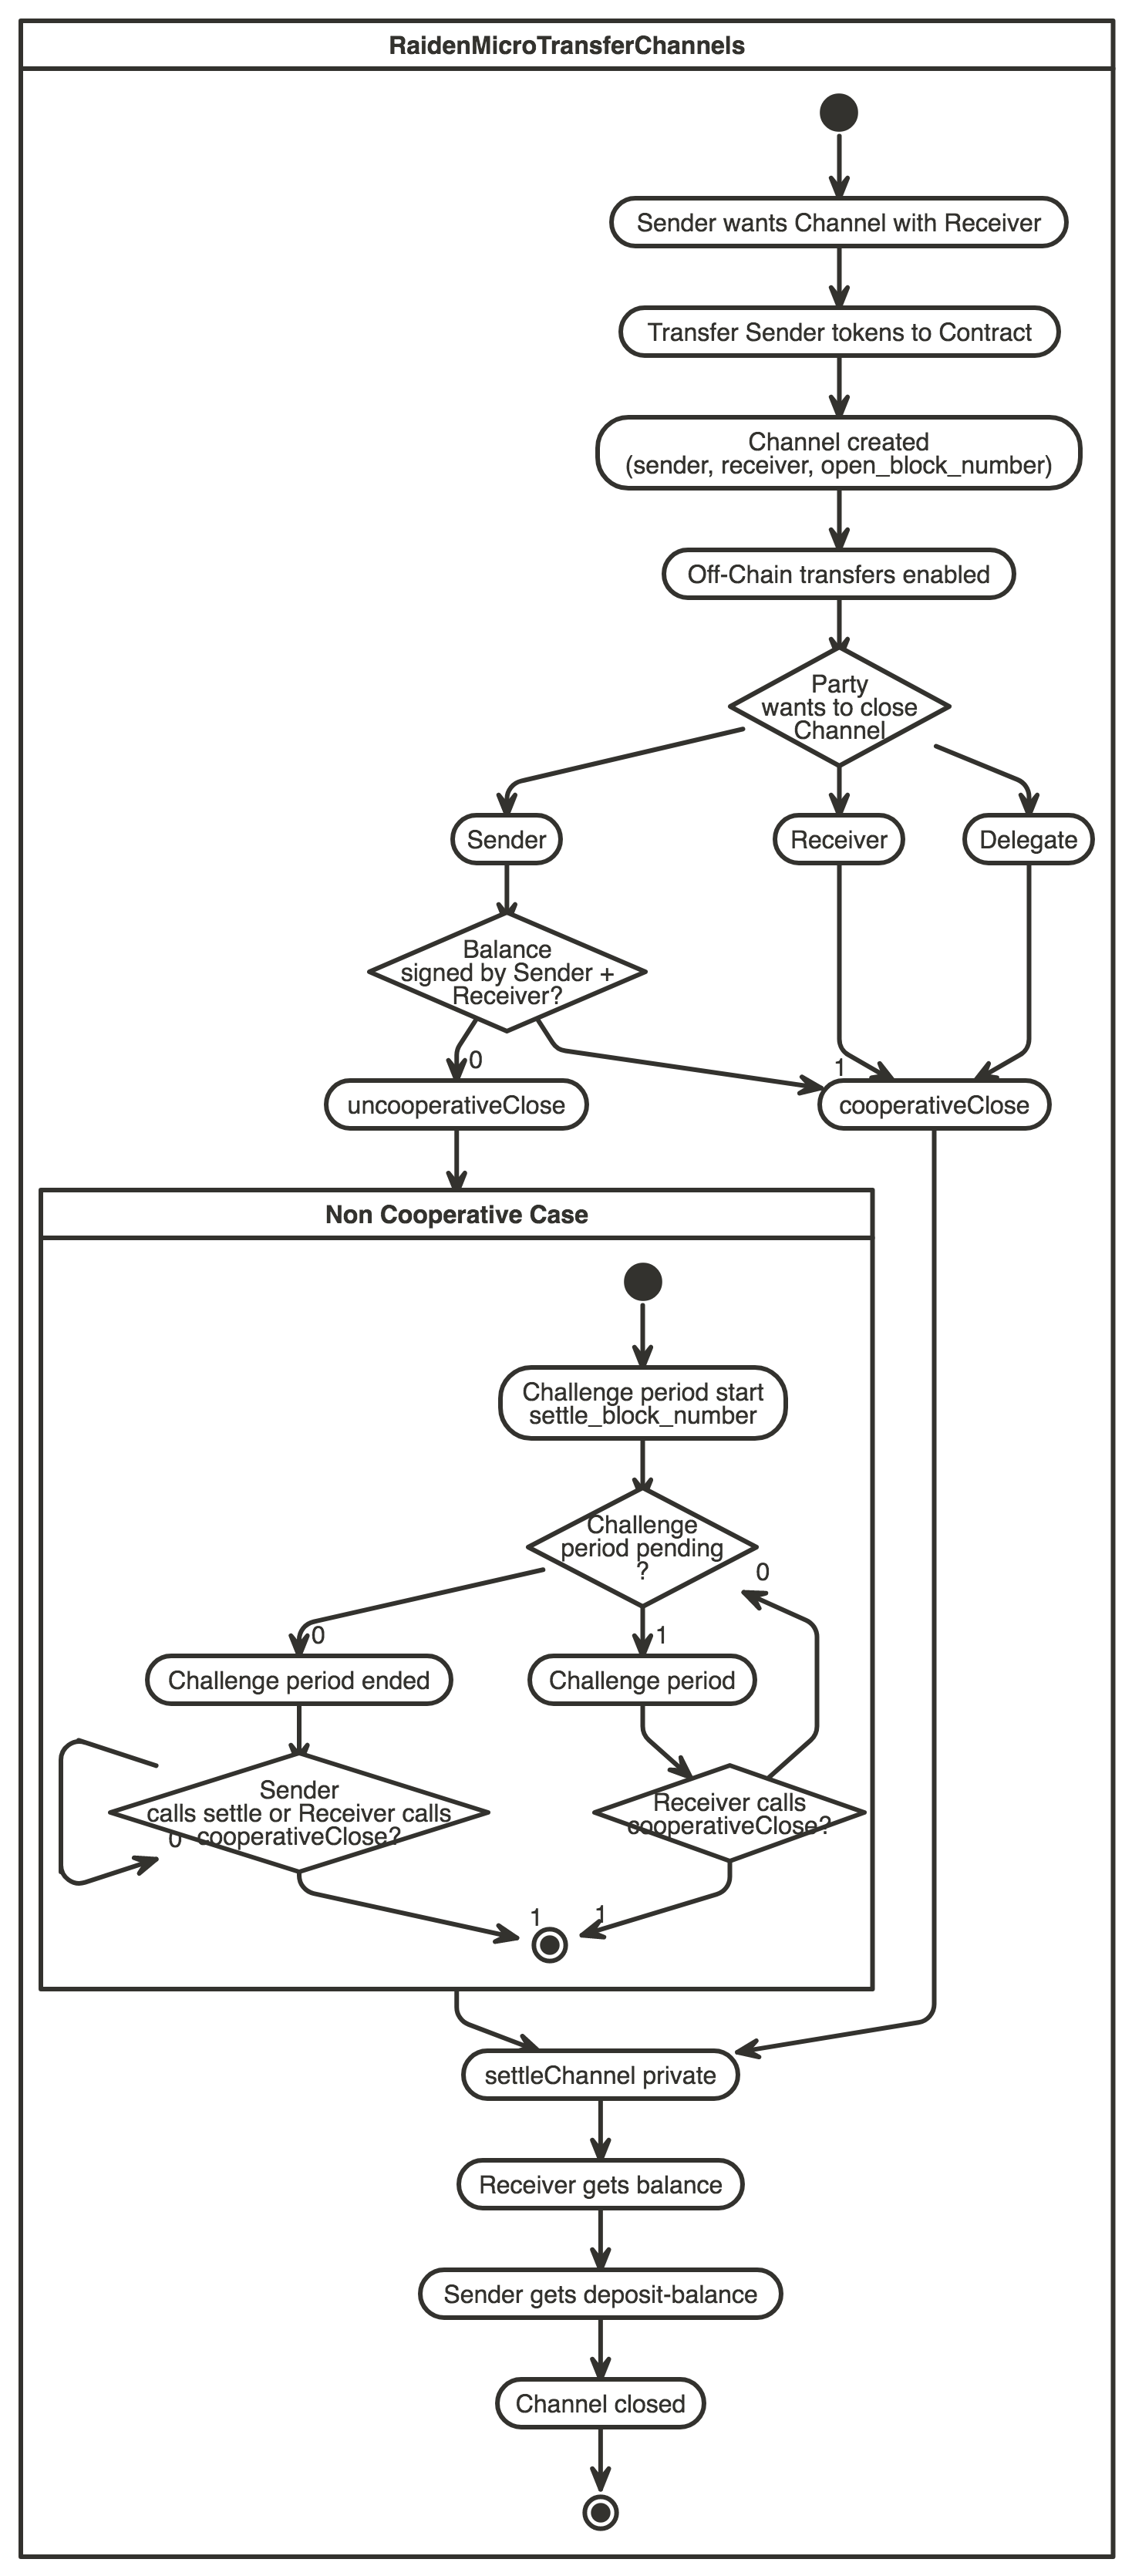
\includegraphics[width=95mm]{image/ChannelCycle.png}
 \caption{μRaidenの取引プロセス}
 \label{ChannelCycle}
\end{figure}
μRaidenはスマートコントラクトを使用しているので、よりフレキシブルにオフチェーン取引中の中間でトークンを引き出すことができる。
また、オンチェーンのトランザクションによってオフチェーンにデポジットしているトークン量を増やすことも可能である。
そしてERC20やERC223に準拠したEthereumネットワーク上で動くトークンに対して全てで動くように設計されている。

\section{まとめ}
この章はブロックチェーン技術全般についての仕組みやその問題点、BitcoinやEthereumの特徴などについて述べた。
途中ではトランザクションの処理の上限を緩和するための技術であるオフチェーン技術についても触れた。
また、Ethereumは最初にブロックチェーンが実装されたBitcoinよりもフレキシブルな非中央集権のコードベースで動く世界を作られる可能性を秘めていることを述べた。
%\chapter{MIWWG:支配者の存在しないIoTデータ市場}
本章では、本研究で提案するIoTデータ市場であるMIWWGについての要件と、そのデータ市場における取引のプロセスについて記述する。
また、MIWWGとは "MIWWG works without governor"を表し、再帰的頭字語を使っている。

\section{MIWWGが達成する目的}
本研究の最終的な目標はオープンなIoTデータ市場の参加者が、参加者自らの意思によってルールや管理団体を設立できるものである。
詳細な理由については4.2.1項にて後述するが、今のクローズドなIoTデータ市場の方式を拡張することでこの理想の実現を目指すことは難しい。
一方で、オープンなIoTデータ市場の方式を拡張することでこの理想の現実を目指すことは可能であると考える。
この時、もっとも最終的な理想の市場を実現するため、もっともオープンな市場を実現することが本研究のMIWWGが達成する目的である。
今後このP2P通信によって構築されたMIWWGを基にした、ルールや管理団体の設立の方法について議論や実装が行われることを期待するものである。

\section{市場の要件}
本節では、前節に記述した達成する目的のため、より具体的に市場が満たすべき要件を述べる。
前半の1~2項に関しては機能要件であり、後半の3~6項に関しては非機能要件である。
前半はMIWWGの基本理念を継承したものであるか否かを測るものとして、後半はMIWWGの評価指標としてMIWWGが改良されて行くこの先も使用されうるものであることを意識して記述した。

\subsection{中央集権装置を必要としない通信モデルによる市場の創造}
本市場において、中央集権組織である管理者の存在はオープンな市場である上でもっとも不要なものである。
管理者は市場を一存で動かせるため、当然ながら巨大な力を持ち得る。
そしてこの大きな力は市場の前提条件を簡単にひっくり返せたり、市場の取引に対する疑義を生じさせる原因となる。
全員が透明に見ることが可能なルールによる支配を行えることにより、この危険性への懸念や疑義を払拭することが出来る。
この中央集権組織支配の排除を目指すとき、既存の代表的なサービス提供方式であるサーバ・クライアント型ではサーバ上でサービスが提供される以上、このサーバの管理者が市場に管理者となってしまい目標の達成が難しい。
そこで例えばP2P通信により、市場の参加者の全員が対等な立場で市場を形成することを考える。
P2P通信は特定の管理者を不必要とするが、このP2P通信上で同意を得た上で管理者にあたるノードを選ぶことは可能である上、P2P通信上でルールやプロトコルを作ることは可能である。
ここで規制が丁度良いルールや管理団体の存在する市場を目指すとき、もっともクライアント・サーバ型を使ったクローズドな市場から目指すことは難しいが、逆にP2P通信型を使ったオープンな市場から目指すことは可能であるという現状が見えてくる。
そしてMIWWGは丁度良い規制の市場を目指す最初の段階として、もっともオープンでルールも管理団体も存在しないIoTデータ市場をP2P通信で実現することを目的としている。
よってMIWWGの機能要件の一つとして、P2P通信を始めとした中央集権装置を必要としない通信モデルによる市場の創造が挙げられる。

\subsection{データの売買}
本市場において、データの売買が可能である必要がある。
ここで売買とは何かを日本国の民法555条から引用して考える。
「売買は、当事者の一方がある財産権を相手方に移転することを約し、相手方がこれに対してその代金を支払うことを約することによって、その効力を生ずる。」
つまり、データ売買に関する取引が成立したとき、データの売り手が買い手へデータを提供する必要がある。
また同時に、買い手は売り手へ代金を支払う必要がある。
そして、これらには契約と同時に上記二つの必要な要件を履行する義務が生じる。
但し、これらは法律的な売買の定義とその解釈であり、実際にデータの売買契約には以下のプロセスが必要となる。
また、今後そのプロセスを遂行するために作られたモジュールを呼ぶための名称を付記する。
\begin{enumerate}
\item 売り手がどのようなデータを売りたいか、またその値段などを示し、データを出品する。データ出品モジュール
\item 買い手が出品されたデータを閲覧する。:出品データ一覧取得モジュール
\item 買い手が閲覧したデータの中から欲しいデータを選び、売り手へ売買契約を申し込む。:売買申し込みモジュール
\item 売り手は申し込まれた契約に対し、応じるか否かの返答をする。:売買契約前確認モジュール
\item 売り手が申し込みに応じた場合、売買契約を成立させる。:売買契約作成モジュール
\item 買い手が売り手へ代金を支払う義務を遂行させる。:支払い義務遂行モジュール
\item 売り手が買い手へデータを転送する義務を遂行させる。:データ転送義務遂行モジュール
\end{enumerate}
以上が必要なプロセスであり、データの売買に必要な要件である。

\subsection{取引に関する秘匿性}
ここでは2点について述べる。
A. データに関して、売り手が意図しない相手へのデータの公開は行わない。
B. 取引の内容について、トークンやデータの取引上必要な情報以外は極力ブロックチェーン上に載せず、公開しない。
まずAについてだが、データは情報商品であり、その情報は一般に入手できないため、価値が存在するものである。
そのデータが本市場の上から意図しないところへ大量に漏れるとすれば、それは本市場がデータの価値を毀損していることにつながり、本市場が意味の少ないものになってしまう。
よってブロックチェーン上へデータを送るなど、マイナーを含む買い手以外の人間に対して売り手が意図しないところでデータが公開されることは避けなければならない。
次にBについてだが、例えばデータを取得するためのアクセス先かアクセス元を公開しなければならないとする。
例えばデータを売り手が買い手へプッシュするのか、買い手が売り手にプルするのかについて議論をしてみる。
この時http(s)通信を使い、 curlなどでデータをプッシュかプルをする際は必ず売り手か買い手がIPアドレスをブロックチェーン上へ暴露しなければならない。
そうでなければ、ノードが見つからないためだ。
ここでは平均して1つの事業者が平均でm個のデータノードを所有しており、1つのデータノードは平均してn個の事業者にデータを売ると考えられる市場を仮定する。
この時、データ受け取り手のIPアドレスを暴露する場合は1人の事業者に対して\(m \times n \)個のIPアドレスを暴露する必要がある。
一方でデータの送り手のIPアドレスを暴露する場合は1人の事業者に対して \(\frac{1}{ m \times n }\)個のアドレスを暴露する必要がある。
するとこの場合、\(m \times n \ge 1\)であればデータの送り手のIPアドレスを暴露する方が、事業者に紐付く情報が少なく済む可能性がある。
勿論、これに関しては作成する市場の目的によって異なる。
また、IPアドレスよりも一時的に使用するために生成されたメールアドレスなどの方が、より秘匿性は高い場合も存在するであろう。
ここでは、取引に関してなるべく他者から秘匿されるべき項目についてあげ、記述を行なった。

\subsection{売買方法の決定可能性}
オープンでルールや支配組織の存在しない市場は、売り手が広場に農作物を持ち寄って勝手に出来上がる市場と同じようなものである。
そこにおいては当然、売り手は好きな方法で好きな値段をつけて商売ができる。
これと同じように、本市場の売買方法はフレキシブルである方が良い。
例えば4.2.2項で記した「支払い義務遂行モジュール」と「データ転送義務遂行モジュール」の二つについて考えてみる。
民法による売買の定義を参照すると、本来は売買契約と同時に、売主の財産権移転義務と買主の代金支払義務は同時履行される。
しかし、データとトークンを同時に一瞬のラグもなく送信し合うことは技術的に難しい。
そこでデータとトークンのどちらを先に送信するかについて議論が起こる。
売り手のデータの到着を確認して、買い手のトークンを送るのか、あるいはその逆か。
後払いを選んだ場合、最初に売り手がデータを投げ、それに対して買い手は支払いを行う。
その後はトークンの移動を売り手が確認してから新しくデータを投げることとなる。
一方で前払いを選んだ場合、最初に買い手がトークンを投げ、それに対して売り手はデータを送る。
その後は買い手は送られてきたデータを確認してから新しいトークンを投げ、必要なデータを取得することとなる。
前払いが良いか後払いが良いかは、売るべきデータの種類に依存すると考えられる。
例えば3秒に1回送信されるデータであり、データが何個も連続して時系列に送られることによって初めて価値のあるデータというものが存在するだろう。
例えば高速道路を定点観察している写真がこのデータの内容である場合だ。
この時は、データに対して後払いを認めた方が得であると考えられる。
何故なら、ユーザはそのデータの内容を見てから、本当に欲しかったデータ形式やデータ内容であるかを精査できるからである。
一方。例えばある地点の気温と湿度のデータを10分に1回送信しているデータノードが存在するとしよう。
この時に後払いを認めてしまうと、一度しか情報が入らない人は常に一度のみのデータを貰い、それに対するデータを払わずに取引を中断してしまう可能性がある。
このように、前払いか後払いかについてでも、データの内容によって売り手の希望は変わってくる。
同じように、何個のデータに対してどれだけのトークンを支払い、支払いのラグはどこまで認めるのかについて売り手がよりフレキシブルに決められることが要件の一つである。

\subsection{大量なIoTデータのリアルタイム処理}
本研究において、IoTデータとは細かい間隔(1~10秒)でリアルタイム流れてくるデータのことを呼ぶ。
蓄積データが対となる概念であり、ある都市の過去1年間の気温データなどはリアルタイムではなく既に存在しているデータであるので、蓄積データと呼ぶ。
これに対し、現在のある都市の気温はリアルタイムで取得できるデータであり、IoTデータと呼ぶ。
このIoTデータの売買を裁くには、大量の処理を裁く必要が出てくる。
少なくとも、PoW(Proof of Work)を基にしたブロックチェーンのオンチェーン技術のみでは裁くことができない。
その場合はオフチェーンを利用することが考えられる。
また、将来的には一部をオンチェーンでPoA(Proof of Authority)を利用し、一部の管理団体がトランザクションを速く裁くことも必要になるかもしれない。
PoAとはトランザクションのマイニングを一部の有資格者が行える仕組みのことで、一定のハッシュパワーでトランザクションの承認が行われる方式である。
この方式は、承認者の数が多いほど捌けるトランザクションの数が増えるという利点を持っている。
一方で、中央集権型の統治へ逆戻りしてしまっている様子も伺える。
オンチェーンやオフチェーン\UTF{00B7}それに関わる政治的な要素は様々あるが、IoTデータというリアルタイムデータを扱う以上、大量データのリアルタイム処理を行えることは要件の一つである。

\subsection{ダウンタイムの非存在}
IoTデータ市場はIoTの発展に伴い、とても大きな市場規模を持つようになる。
データ市場に限らない数値であるが、2022年のIoT市場規模は11.7兆円と言われている。(http://www.itmedia.co.jp/enterprise/articles/1809/13/news132.html)
このようなプラットフォーム上で大きな価値のあるアプリケーションが動いている場合は、ダウンタイムが起きると多額の損害が生まれてしまう。
その状況の中で、2章で述べたようにAWSのSLAは99.99\%であり、年間では52.56分落ちている可能性があるのだ。
そのわずか一時間弱の間であっても、IoTデータ市場の規模の大きさを考えるとダウンタイムは看過できない。
また機械的のハードウェア的な故障のみならず、人為的なバグや人為的なオペレーションミスも一つのサーバ上でサービスが動いている場合は考えうる。
そこでP2P通信を始めとした方法で、ある事業者のサーバが壊れてもネットワーク全体には影響を及ぼしにくいサービスモデルであることが望ましい。
P2P通信であることは要件にはならないが、ダウンタイムの存在がほぼ否定されるほど、この市場が動くネットワークがダウンタイムを起こしにくくすることは要件の一つである。

\section{取引のプロセス}
本節では、MIWWGにおけるIoTデータ取引のプロセスを示す。

\subsection{データ陳列}
最初に、データの売り手が自分の持っているデータの種類をMIWWGネットワーク上へ公開する。
この際、取引に必要な事項である値段やデータが送信される間隔といった値を同時に提出する。
しかしデータについての詳細な説明書きや例を大量の文字によって記述する場合があった場合、マイナーへ大きな量の手数料を払う必要が生じる。
その際はデータに関する詳細を記述したURLを記述し、そのURLに詳細なデータに関する記述を行うという方法を取ることも可能である。
売り手は自身の持つデータをブロックチェーン上へと送信し、これがブロックに含まれた瞬間からデータが全ノードへと知れ渡ることとなる。

\subsection{取引開始}
次に、買い手が陳列されたデータを閲覧し、必要なデータについて取引を開始する。
この時、一般的なオフチェーン技術の特徴から、買い手は今後どの程度の期間でそのデータが必要であるかについて考慮し、その期間の間に使われる分のトークン量をデポジットする必要がある。
このデポジットについては、相手の同意のない限りデータの買い手側が即座に引き出すことはできない。
取引開始のトランザクションをブロックチェーン上へ送信し、それがブロックに含まれた瞬間が取引開始の瞬間である。
トランザクションがブロックに含まれた後、http(s)通信などによってデータを読み込む際のIDとパスワードをデータの販売元へ送信する必要がある。

\subsection{データ販売とトークン転送}
本項を含む、オフチェーンの文脈においてトークンの転送とは、買い手がそのトークンバランスに同意したことを示す署名値を売り手へ送信することである。
取引開始後、トークンが買い手から売り手へとデータの送信間隔と同じ間隔で送信される。
データ転送を売り手が止めた場合、買い手はトークンの転送を止める。
逆に、トークンの転送を買い手が止めた場合は、売り手はデータ転送を止める。
この際、故意に転送を止めた場合でなくとも、ネットワークの一時的な不通によってデータやトークンの転送が行われなかった場合も同様に相手側は取引を停止する。
従って、データ陳列の際にどの程度の支払いの遅れまでを売り手が許容するかという内容や、売り手のネットワーク状況によってどの程度のデータ転送の遅れまでを買い手が許容するかという内容についてをデータ陳列の際に記述しておくべきである。
このデータ転送はhttp(s)通信によって行われ、ブロックチェーンネットワークとは全く関係のない動きをする。
従って、これらのデータ販売や転送はブロックチェーンの処理能力に囚われない。

\subsection{取引終了}
買い手がトークンの転送をやめた場合や売り手がデータの転送をやめた場合は取引の途中であっても取引が終了する場合がある。
逆に、デポジットの全ての転送が終わった場合はデータの売り手によって取引は終了される。
いずれでも、買い手か売り手が取引終了に関するトランザクションがブロックチェーンネットワークに送信することで、取引は終了を迎える。

\section{まとめ}
本章に記述したプロセスを一つの図で示したものが以下の図\ref{process}である。
買い手と売り手がどちらも取引終了を主張した場合のプロセスを示している。
\begin{figure}[htbp]
 \centering
  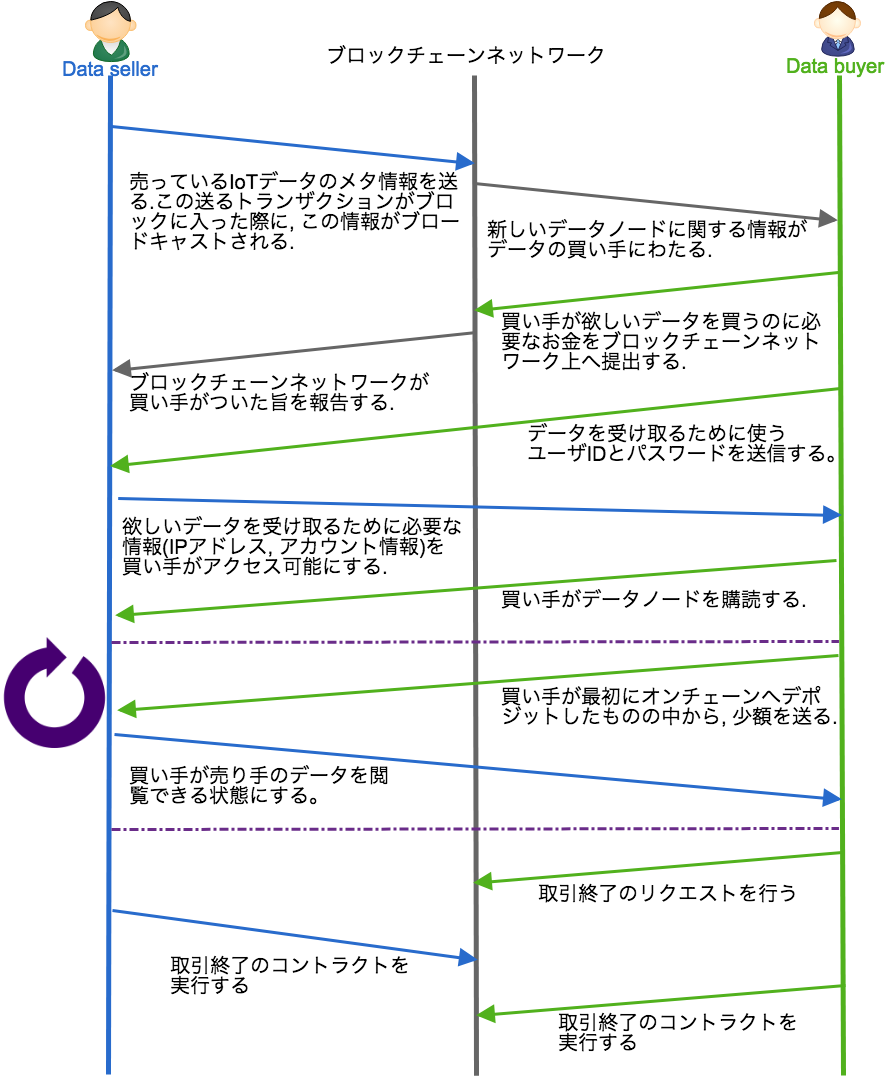
\includegraphics[width=140mm]{image/process.png}
 \caption{MIWWGの取引プロセス}
 \label{system}
\end{figure}


%\chapter{設計と実装}
本章では, 前章にて述べたMIWWGを実現する際の設計と実装について述べる。
また、本研究においては大きく分けて3つの技術を用いている。
市場における貨幣の役割を担うブロックチェーン技術、そのブロックチェーン技術の弱点であるトランザクション流通量の上限を引き上げるオフチェーン技術、IoTデータを実際に送信する役割のメッセージングシステム技術の3つである。
これら3つのうち各々をどのように用いたかについて、独立した節にて説明を行う。

\section{設計}
最初に、本節では設計について述べる。
\subsection{システム構成}
以下に、システム設計図\ref{SystemDesign}を示す。\\
\begin{figure}[htbp]
 \centering
  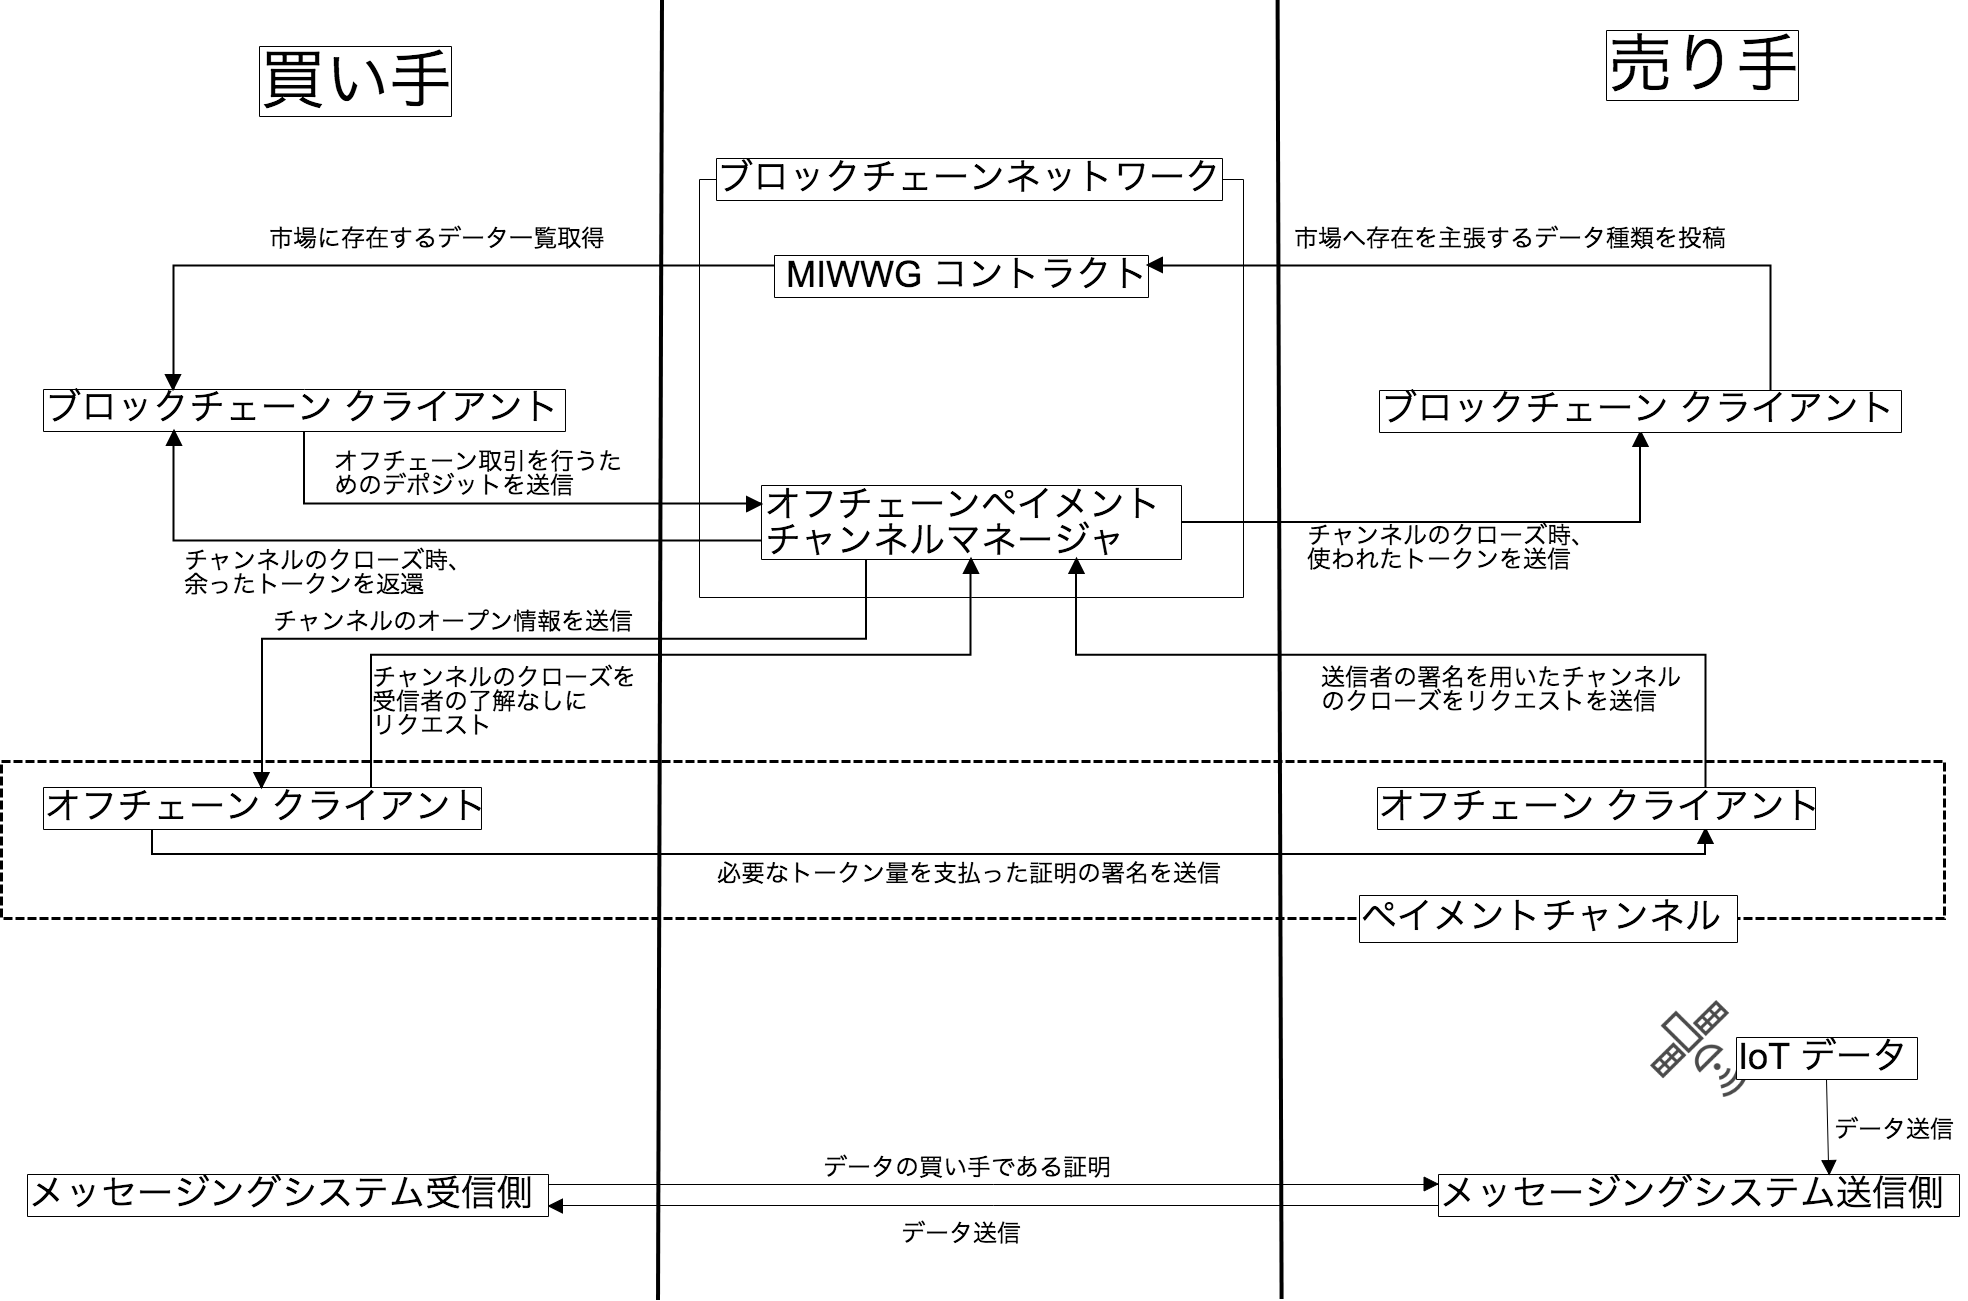
\includegraphics[width=160mm]{image/SystemDesign.png}
 \caption{システム設計図}
 \label{SystemDesign}
\end{figure}

\subsection{ブロックチェーン技術}
本研究において、ブロックチェーンのトークンが貨幣の役割を担い、ブロックチェーンはその元帳の役割を持つ。
一般に、ブロックチェーンはコントラクトを生成することが出来る。
そのコントラクト上にて、市場に存在するデータの管理やトークンの移動を行う。
データに関する情報のうち、多くの人にとって重要な定量的情報を列挙し、それをコントラクトの中に記述する。
本研究では以下の項目を定量的情報として入力させることとした。

\begin{itemize}
\item データの名前
\item 1つのデータあたりの値段
\item データが送られてくる間隔
\item トークン送信の遅延に関する許容時間
\item 前払いで必要なトークンの量
\item データの売り手のアドレス
\item データに関するその他の説明がある場合、それを記述するURL
\end{itemize}

1つのデータあたりの値段とデータが送られてくる間隔、データの売り手のアドレスはデータの買い手がトークンを利用する際に必要な情報である。
また、買い手が環境の悪いネットワーク環境下からデータを買おうとする場合、トークン送信の遅延に関する許容時間は重要なファクターとなる。
買い手に契約を終了する気持ちがなくとも、売り手がトークン送信の見送信を検知し、契約が終了となる可能性があるためである。
その場合、もう一度契約をオンチェーンの処理によって開始する必要があり、これは本来不必要であったマイナーへの手数料を必要とする。
前払いで必要なトークンの量は、契約を開始した後に直ぐに買い手がトークンを未送信にしてしまい、買い手がデータを遅延の許容時間分だけ無料で受信するのみで契約を終了してしまう行動を抑制するためのものである。
また、これらの定量的情報以外にデータに関する詳細な説明を記述する場合は、そのデータに関する情報を記載したURLをトランザクション内に記述する。
このことにより、このデータの存在を市場へ主張する際のトランザクションサイズを小さくする狙いがある。
一方、同じURLであってもそこに記載する内容はブロックに入った後も変更可能である。
従って、取引における重要な事項をこのURLに記述したとしても、それは信頼できるものではない。
あくまでURLの記述内容は他の項目にプラスして、データに関する内容を理解するために使われるものとなる。

\subsection{オフチェーン技術}
本研究において、オフチェーン技術はブロックチェーンの処理能力を補完するために使われる。
IoTデータは短い時間間隔で流れてくるデータであり、ブロックチェーンの処理能力では追いつかないためだ。
データ取引の開始時にオンチェーンにてデポジットを行い、ペイメントチャンネルをオープンし、その情報がオフチェーンクライアントへ渡る。
そしてデータの買い手は売り手へ新しいトークンバランスによる署名値を提出することで、データの売り手へトークンを渡す。
最後に、データの買い手か売り手のいずれかがチャンネルをクローズし、最終的にデポジットされたトークンを分配する。

\subsection{メッセージングシステム}
本研究において、メッセージングシステムはIoTデータの送信に使われる。
一般に、メッセージキューシステムに基づく分散メッセージングシステムは次のような特徴を持つ。
\begin{itemize}
\item 非同期のメッセージ送信が可能である。これにより送信側と受信側とのサービスが疎結合になり、片方の処理の遅延がもう一方に影響を与えるリスクが減る。
\item 送信を行う一つのノードが落ちたとしても、他のノードが直ぐに落ちたノードの代わりの役目を担う。これにより、可用性が高いことが担保される。
\item 送信側で新しくノードを追加した時、新規ノードを含めた協調動作が始まる。これにより、拡張性が高いことが担保され、より多くのメッセージ処理を裁くことが出来るような拡張を簡単にすることが出来る。
\end{itemize}
これらの特徴から、今回のIoTデータ市場の構築にはメッセージングシステムを使うことは最適である。
送信者と受信者のシステムが疎結合であり、各々の責任によってデータの送受信が可能なためだ。
また、メッセージングシステムによってはCAPの定理においてどの要素を重視するかをパラメタで指定することも可能であり、データの送受信者にとってよりフレキシブルな設定が可能となっている。\\
また、メッセージングシステムはkerberosや簡単なユーザID/パスワード認証などを用い、データの買い手のみへデータの提供をしなくてはならない。
そしてトークンの取引が停止されたことが検知された時からなるべく早く、データの送信を不許可にしなくてはならない。

\subsection{実装}
\subsection{システム構成}
以下に、システム構成図\ref{SystemImplement}を示す。\\
\begin{figure}[htbp]
 \centering
  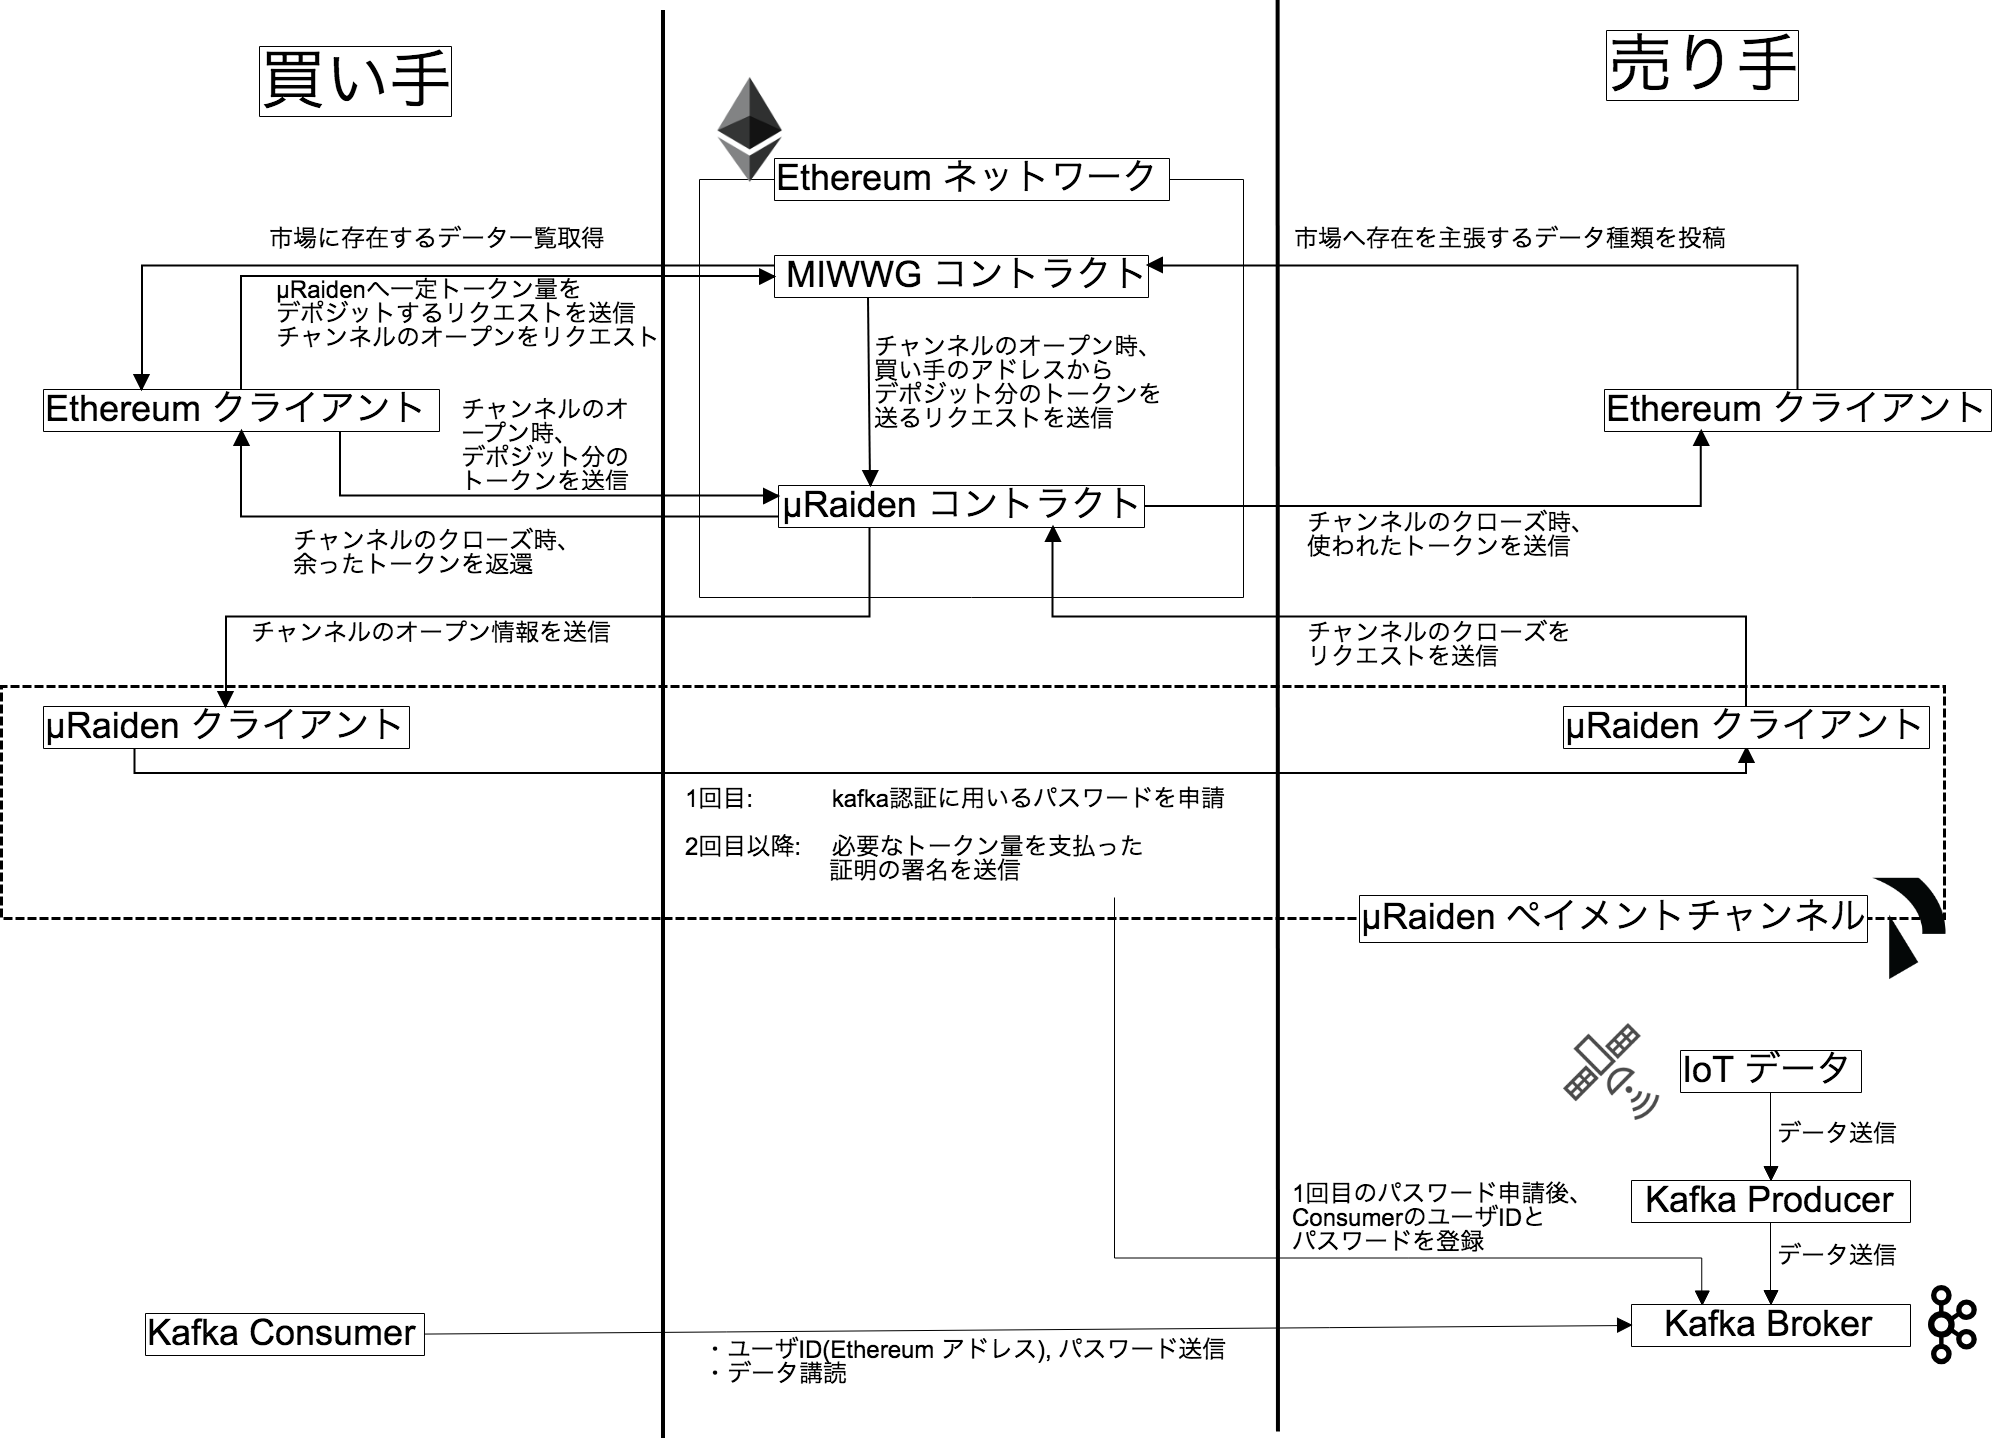
\includegraphics[width=160mm]{image/SystemImplement.png}
 \caption{システム構成図}
 \label{SystemImplement}
\end{figure}

\subsection{ブロックチェーン技術}
本研究では、ブロックチェーン技術の中からEthereumを利用する。
また、そのEthereumクライアントとして、go言語による実装であるgo-ethereum(以下、geth)を利用した。
ここでgethのオリジナルコードとは、gethのgithubレポジトリ(https://github.com/ethereum/go-ethereum)のConstant (v1.8.20)のことである。
solidityは0.4.17のバージョンを利用している。
最初に開発したトークンの中身について記述する。
採用したトークン規格はERC20に次ぐトークンの規格であるERC223を考慮しつつ、一部を改変して利用した。
これはERC223が本研究で採用するオフチェーン技術であるμRaidenがより薦める方式であるためである。
既存のERC20と比べて、コントラクトアドレスに対して誤ってトークンを送った時に取り戻せるtokenFallback関数が追加され、コントラクトに対するトランザクションとユーザに対するトランザクションを同じように捌けるようになっている。
これによりEthereumの掲げる理想である相手がコードか人間か気にせずにトークンのやり取りが出来るという世界をより体現しているものである。
このERC223の一般的な実装物はgithubのレポジトリであるDexaran/ERC223-token-standard(https://github.com/Dexaran/ERC223-token-standard)に存在する。
この元のソースコードに加える形で本研究では以下の構造体によってIoTデータを格納可能とした。
\begin{lstlisting}[caption=solidityによるデータを保持する構造体,label=DataNode]
struct DataNode {
  string name;  // データの名前
  uint256 price;  // 1つのデータあたりの値段
  uint256 interval;  // データが送られてくる間隔
  uint256 delay_permission_time;  // トークン送信の遅延に関する許容時間
  uint256 prepaid_value;  // 前払いで必要なトークンの量
  address author;  // データの売り手のアドレス
  string explanation_url;  // データに関するその他の説明がある場合、それを記述するURL
  uint256 data_index;  // 本データがデータ市場において一意に定まるID。1から順番にインクリメントされていく。
}
\end{lstlisting}
以上がIoTデータの種類を格納する構造である。
また、この他にEthereumトークンを本トークンへ変換することのできる機能を実装した。本トークンはEthereumの1wei = 1MI(本トークンの通貨単位)としてEthereumネットワーク上で動くものである。
さらに、一般的なtransfer(\_to, \_value, \_data)の関数をラップするbuyData関数を作ることによって、μRaidenクライアントから何のデータを買いたいかについて、買い手からの情報を得る実装を行なっている。以下がその様子である。
\begin{lstlisting}[caption=gethのEIP155のフォーク確認機能の削除 params/config.go ,label=DataNode]
uint256[] user_bought_log; // ユーザの購入履歴を格納
function buyData(
    address _to,
    uint256 _value,
    bytes _data,
    uint256 data_index)
    public
    returns (bool)
{
    user_bought_log.push(data_index); // ユーザの購入履歴に追加
    emit boughtData(msg.sender, data_index);  // ユーザの購入が行われたことを示すeventを送出
    bool ret = transfer(_to, _value, _data);  // ERC223対応のtransfer関数を実行
    return ret
    }
\end{lstlisting}
これにより、一つのトランザクションによってデータの購買とそれに関するペイメントチャンネルを開くという二つの行為ができるようになっている。 \\
次に今回使用したgethに加えた変更について述べる。
今回はプライベートネットワークで動作を検証するにあたり、gethがμRaidenの発行するEIP155を考慮した署名のトランザクションを捌かないという事象が発生した。
これはリプレイアタックを防ぐためのものであり、Ethereumのブロックナンバーが2675000以降のものについてのみEIP155を適用する実装がなされていた。
しかし、これではトランザクションが裁かれ始めるまでに大量の時間を要してしまうため、この機能を簡単に削除した。
\begin{lstlisting}[caption=gethのEIP155のフォーク確認機能の削除 params/config.go ,label=EIP155]
227 // IsEIP155 returns whether num is either equal to the EIP155 fork block or greater.
228 func (c *ChainConfig) IsEIP155(num *big.Int) bool {
229     //return isForked(c.EIP155Block, num) // 既存の判別箇所を削除
230     return true // 全てのEIP155署名のトランザクションが裁かれるように変更
231 }
\end{lstlisting}

\subsection{オフチェーン技術}
オフチェーン技術について、本研究ではμRaiden(https://github.com/raiden-network/microraiden)の0.2.0を使用した。
このμRaidenについて、いくつかの変更を加えている。
最初に、ペイメントチャンネルをオープンするためにMIWWGコントラクトへtransfer関数を実行する際、独自の関数であるbuyData関数を呼び出している。
\begin{lstlisting}[caption=μRaidenクライアントの変更 client/client.py  ,label=RaidenOpenChannel]
def open_channel(self, receiver_address: str, deposit: int):
    data = decode_hex(self.context.address) + decode_hex(receiver_address)
    tx = create_signed_contract_transaction(
        self.context.private_key,
        self.context.token,
        # 'transfer', //オリジナル部分
        'buyData', // 追加部分
        [
            self.context.channel_manager.address,
            deposit,
            data,
            data_index // 追加部分
        ]
    )
\end{lstlisting}
上記と同じ変更をペイメントチャンネルへのデポジットを増やす際に使用するtopup関数にも加えている。
また、デフォルトの設定で用いるとethereumのテストネットワークへと繋がってしまい、プライベートネットワークに繋がらない。
よって以下の変更を加えた。
\begin{lstlisting}[caption=ネットワーク設定の変更 config.py  ,label=RaidenOpenChannel]
 40 # network-specific configuration
 41 NETWORK_CONFIG_DEFAULTS = {
 ...
 63     # private MIWWG //63行目から67行目まで追加部分
 64     98: NetworkConfig(
 65         channel_manager_address='0xd0c19d7d41ae4a5561d2289d997da00b9de1bf73',
 66         start_sync_block=0
 67     ),
 ...
104    #NETWORK_CFG.set_defaults(3)  // デフォルトのネットワークID
104    NETWORK_CFG.set_defaults(98)  // 今回使用するネットワークID
\end{lstlisting}
また、μRaidenはバックエンドのDBとしてsqliteを使用している。
このDBを使って、のちにメッセージングシステムにてユーザIDとパスワードを使用した認証を行う。
そのパスワードを保持する目的と、μRaidenでは想定されていない同じ送り手と受取り手のアドレスに対して複数の別のペイメントを使用することから、DB構造について変更を加えている。
\begin{lstlisting}[caption=DB構造の変更 channel\_manager/state.py  ,label=sqliteSql]
CREATE TABLE `channels` (
    `sender`            CHAR(42)        NOT NULL,
    `data\_index`            INTEGER        NOT NULL,  # 追加
    `password`            CHAR(42)        NOT NULL,  # 追加
    `open_block_number` INTEGER         NOT NULL,
    `deposit`           DECIMAL(78,0)   NOT NULL,
    `balance`           DECIMAL(78,0)   NOT NULL,
    `last_signature`    CHAR(132),
    `settle_timeout`    INTEGER         NOT NULL,
    `mtime`             INTEGER         NOT NULL,
    `ctime`             INTEGER         NOT NULL,
    `state`             INTEGER         NOT NULL,
    `confirmed`         BOOL            NOT NULL,
    PRIMARY KEY (`sender`, `open_block_number`, `data_index`)  # 最後の要素について、追加
);
\end{lstlisting}
またこれに伴い、このDBを利用するコードについても全て変更を加えている。
他の機能として、パスワードを登録する際にアクセスするapiのエンドポイントを作成している。
WebサーバはgeventのpywsgiにあるWSGIServerを用い、その上でflaskを使い、ルーティングを行なっている。

\subsection{メッセージングシステム}
本実装では、JVM上にて動作するkafkaをメッセージングシステムとして用いている。
kafkaはconsumerとbroker, producerからなり、各々がデータの受け手、コーディネイター、送り手である。
各々でクラスターが構成可能で、可用性に優れたメッセージングシステムであるため、本研究にて用いた、
バージョンであるが、このkafka内におけるSASL\_PLAIN認証を用いてユーザ認証を行うものの、現状の最新バージョンである2.1.0や2.0.0ではこの認証が動作しなかった。
したがってメジャーダウングレードを行い、1.0.2のバージョンを用いている。
また、scalaは2.12のバージョンを用いている。
そしてユーザ認証は以下のconfファイルを用いたSASL認証を使用している。
\begin{lstlisting}[caption=SASL認証の設定 config/producer.properties  ,label=serverProperties]
sasl.mechanism=PLAIN
security.protocol=SASL_PLAINTEXT
sasl.jaas.config=org.apache.kafka.common.security.plain.PlainLoginModule required \
  username="yoshiyuki" \
  password="yoshiyuki-secret";
\end{lstlisting}
また、JVMを立ち上げた後でも、このファイルにユーザ記述部分を足すことでkafkaへ動的にユーザの追加が出来る。
これにより、新しいユーザの追加を行っている。
また、シェルを経由してbin/kafka-acls.shを用いることで動的にユーザの権限の制限が可能となる。
これにより、トークンを送信してこなくなったユーザからデータを購読する権限を剥奪している。 \\
また、kafkaはCAPの定理におけるCAを満たすものであり、PであるPartition Tolerance(分断耐性)は低いものである。
これについて、kafkaは本来は同一データセンター内にて用いられることが前提のプロダクトであり、分断される可能性が低いので問題ないとしている。
しかし、今回のユースケースではkafkaのproducerとconsumerは同一データセンター内に存在しないことの方が多い。
つまり、ネットワークが分断される可能性は十分に考えられるのだ。
そこでacksというパラメタが設定できる。
ここではレプリケーションされたメッセージがいくつ送信成功することを要求するかを指定でき、これにallを指定すると全てのレプリケーションを格納するbrokerに情報が書き込まれることを、producerが要求することとなる。
さらにreplication.factorによってそのメッセージをいくつのbrokerが持つかについて指定することができる。
これらをallや大きな数字に設定を行うと、あるbrokerとconsumerの分断が起こったとしても他のネットワークを用いてデータの配信は可能なままである。
このように、kafkaではAのAvailability(可用性)を犠牲にすることでPの分断耐性を増すことが可能であり、今回のユースケースではPを増すことを考慮する必要がある。

\section{まとめ}
本章では本研究にて用いるブロックチェーン技術や、それをIoTデータのような短い間隔の支払いが必要な場合に対応するためのオフチェーン技術、そしてデータを多くのスループットで拡張性を保持しつつ送受信するメッセージングシステムについて述べた。
%\input{6.tex}
%  \newcommand{\fulltoday}{\number\day\space \ifcase\month\or
    January\or February\or March\or April\or May\or June\or
    July\or August\or September\or October\or November\or December\fi
    \space\number\year}

\chapter*{謝辞}
%get rid of * to put it in the table of contents
本研究を進めるにあたり、ご指導を頂きました慶應義塾大学環境情報学部准教授中澤仁博士に深く感謝致します。

また、慶應義塾大学 政策・メディア研究科特任准教授 米澤拓郎博士には、本論文の執筆に当たって御助言を賜りました事を深く感謝致します。
学部1年の時よりお世話になり、直接頂いた言葉以外でも、ミーティングなどで米澤先生の仰る指摘や考え方は参考になりました。
本論文についても、教えて頂いた考え方や研究のやり方を念頭に置きつつ、書き進めて参りました。

そして、私が2年ほどインターンをさせて頂きました、株式会社INTHEFORESTの代表取締役である冨田和孝さんに感謝致します。
本研究の実装のようにオープンソースを使うのみではなく、その中身を理解し、それを変更して自分の作りたいものを作る考えは冨田さんの会社でインターンをさせて頂いたから出来たことであると思っています。
また、明らかに給料に見合わない成果しかあげない私を辛抱強く雇ってくださったことにも感謝します。
大学生活に必要なお金を頂きつつ、実装力をあげられた御社でのインターンがあったからこそ、今回の実装物が作り上げられたと思っております。

また、徳田研究室、中澤研究室において一緒に研究活動を行った先輩・同期・後輩に感謝を致します。

最後に、大学生活の4年間を私が一切の不自由なく過ごせるようにしてくださった家族に感謝を申し上げます。

\begin{flushright}
\fulltoday\\
井上 義之
\end{flushright}


\bibliography{bib.bib}

\appendix

\end{document}